\documentclass[twoside]{book}

% Packages required by doxygen
\usepackage{fixltx2e}
\usepackage{calc}
\usepackage{doxygen}
\usepackage[export]{adjustbox} % also loads graphicx
\usepackage{graphicx}
\usepackage[utf8]{inputenc}
\usepackage{makeidx}
\usepackage{multicol}
\usepackage{multirow}
\PassOptionsToPackage{warn}{textcomp}
\usepackage{textcomp}
\usepackage[nointegrals]{wasysym}
\usepackage[table]{xcolor}

% Font selection
\usepackage[T1]{fontenc}
\usepackage[scaled=.90]{helvet}
\usepackage{courier}
\usepackage{amssymb}
\usepackage{sectsty}
\renewcommand{\familydefault}{\sfdefault}
\allsectionsfont{%
  \fontseries{bc}\selectfont%
  \color{darkgray}%
}
\renewcommand{\DoxyLabelFont}{%
  \fontseries{bc}\selectfont%
  \color{darkgray}%
}
\newcommand{\+}{\discretionary{\mbox{\scriptsize$\hookleftarrow$}}{}{}}

% Page & text layout
\usepackage{geometry}
\geometry{%
  a4paper,%
  top=2.5cm,%
  bottom=2.5cm,%
  left=2.5cm,%
  right=2.5cm%
}
\tolerance=750
\hfuzz=15pt
\hbadness=750
\setlength{\emergencystretch}{15pt}
\setlength{\parindent}{0cm}
\setlength{\parskip}{0.2cm}
\makeatletter
\renewcommand{\paragraph}{%
  \@startsection{paragraph}{4}{0ex}{-1.0ex}{1.0ex}{%
    \normalfont\normalsize\bfseries\SS@parafont%
  }%
}
\renewcommand{\subparagraph}{%
  \@startsection{subparagraph}{5}{0ex}{-1.0ex}{1.0ex}{%
    \normalfont\normalsize\bfseries\SS@subparafont%
  }%
}
\makeatother

% Headers & footers
\usepackage{fancyhdr}
\pagestyle{fancyplain}
\fancyhead[LE]{\fancyplain{}{\bfseries\thepage}}
\fancyhead[CE]{\fancyplain{}{}}
\fancyhead[RE]{\fancyplain{}{\bfseries\leftmark}}
\fancyhead[LO]{\fancyplain{}{\bfseries\rightmark}}
\fancyhead[CO]{\fancyplain{}{}}
\fancyhead[RO]{\fancyplain{}{\bfseries\thepage}}
\fancyfoot[LE]{\fancyplain{}{}}
\fancyfoot[CE]{\fancyplain{}{}}
\fancyfoot[RE]{\fancyplain{}{\bfseries\scriptsize Generated on Sun May 10 2015 22\+:16\+:51 for F\+N\+N++ by Doxygen }}
\fancyfoot[LO]{\fancyplain{}{\bfseries\scriptsize Generated on Sun May 10 2015 22\+:16\+:51 for F\+N\+N++ by Doxygen }}
\fancyfoot[CO]{\fancyplain{}{}}
\fancyfoot[RO]{\fancyplain{}{}}
\renewcommand{\footrulewidth}{0.4pt}
\renewcommand{\chaptermark}[1]{%
  \markboth{#1}{}%
}
\renewcommand{\sectionmark}[1]{%
  \markright{\thesection\ #1}%
}

% Indices & bibliography
\usepackage{natbib}
\usepackage[titles]{tocloft}
\setcounter{tocdepth}{3}
\setcounter{secnumdepth}{5}
\makeindex

% Hyperlinks (required, but should be loaded last)
\usepackage{ifpdf}
\ifpdf
  \usepackage[pdftex,pagebackref=true]{hyperref}
\else
  \usepackage[ps2pdf,pagebackref=true]{hyperref}
\fi
\hypersetup{%
  colorlinks=true,%
  linkcolor=blue,%
  citecolor=blue,%
  unicode%
}

% Custom commands
\newcommand{\clearemptydoublepage}{%
  \newpage{\pagestyle{empty}\cleardoublepage}%
}


%===== C O N T E N T S =====

\begin{document}

% Titlepage & ToC
\hypersetup{pageanchor=false,
             bookmarks=true,
             bookmarksnumbered=true,
             pdfencoding=unicode
            }
\pagenumbering{roman}
\begin{titlepage}
\vspace*{7cm}
\begin{center}%
{\Large F\+N\+N++ \\[1ex]\large 1 }\\
\vspace*{1cm}
{\large Generated by Doxygen 1.8.9.1}\\
\vspace*{0.5cm}
{\small Sun May 10 2015 22:16:51}\\
\end{center}
\end{titlepage}
\clearemptydoublepage
\tableofcontents
\clearemptydoublepage
\pagenumbering{arabic}
\hypersetup{pageanchor=true}

%--- Begin generated contents ---
\chapter{Namespace Index}
\section{Namespace List}
Here is a list of all documented namespaces with brief descriptions\+:\begin{DoxyCompactList}
\item\contentsline{section}{\hyperlink{namespacefnn}{fnn} \\*Different sigmoid activation functions. }{\pageref{namespacefnn}}{}
\end{DoxyCompactList}

\chapter{Hierarchical Index}
\section{Class Hierarchy}
This inheritance list is sorted roughly, but not completely, alphabetically\+:\begin{DoxyCompactList}
\item \contentsline{section}{fnn\+:\+:Data\+Point}{\pageref{structfnn_1_1_data_point}}{}
\item \contentsline{section}{fnn\+:\+:Data\+Set}{\pageref{classfnn_1_1_data_set}}{}
\item \contentsline{section}{fnn\+:\+:Experiment}{\pageref{classfnn_1_1_experiment}}{}
\item \contentsline{section}{fnn\+:\+:F\+N\+N\+Trainer}{\pageref{classfnn_1_1_f_n_n_trainer}}{}
\item \contentsline{section}{fnn\+:\+:Log}{\pageref{classfnn_1_1_log}}{}
\item \contentsline{section}{fnn\+:\+:Loggable}{\pageref{classfnn_1_1_loggable}}{}
\begin{DoxyCompactList}
\item \contentsline{section}{fnn\+:\+:Network}{\pageref{classfnn_1_1_network}}{}
\end{DoxyCompactList}
\item \contentsline{section}{fnn\+:\+:Log\+Manager}{\pageref{classfnn_1_1_log_manager}}{}
\item \contentsline{section}{fnn\+:\+:Math}{\pageref{classfnn_1_1_math}}{}
\item \contentsline{section}{fnn\+:\+:Sigmoid}{\pageref{classfnn_1_1_sigmoid}}{}
\item \contentsline{section}{fnn\+:\+:Weight\+Surface}{\pageref{classfnn_1_1_weight_surface}}{}
\end{DoxyCompactList}

\chapter{Class Index}
\section{Class List}
Here are the classes, structs, unions and interfaces with brief descriptions\+:\begin{DoxyCompactList}
\item\contentsline{section}{\hyperlink{structfnn_1_1_data_point}{fnn\+::\+Data\+Point} }{\pageref{structfnn_1_1_data_point}}{}
\item\contentsline{section}{\hyperlink{classfnn_1_1_data_set}{fnn\+::\+Data\+Set} }{\pageref{classfnn_1_1_data_set}}{}
\item\contentsline{section}{\hyperlink{classfnn_1_1_experiment}{fnn\+::\+Experiment} }{\pageref{classfnn_1_1_experiment}}{}
\item\contentsline{section}{\hyperlink{classfnn_1_1_f_n_n_trainer}{fnn\+::\+F\+N\+N\+Trainer} \\*The Trainer for the \hyperlink{classfnn_1_1_network}{Network} }{\pageref{classfnn_1_1_f_n_n_trainer}}{}
\item\contentsline{section}{\hyperlink{classfnn_1_1_log}{fnn\+::\+Log} \\*A log. }{\pageref{classfnn_1_1_log}}{}
\item\contentsline{section}{\hyperlink{classfnn_1_1_loggable}{fnn\+::\+Loggable} \\*A loggable. }{\pageref{classfnn_1_1_loggable}}{}
\item\contentsline{section}{\hyperlink{classfnn_1_1_log_manager}{fnn\+::\+Log\+Manager} \\*Manager for logs. }{\pageref{classfnn_1_1_log_manager}}{}
\item\contentsline{section}{\hyperlink{classfnn_1_1_math}{fnn\+::\+Math} \\*The main mathematics helper class for F\+N\+N\+L\+I\+B }{\pageref{classfnn_1_1_math}}{}
\item\contentsline{section}{\hyperlink{classfnn_1_1_network}{fnn\+::\+Network} \\*The main class of operation on the functional neural networks. }{\pageref{classfnn_1_1_network}}{}
\item\contentsline{section}{\hyperlink{classfnn_1_1_sigmoid}{fnn\+::\+Sigmoid} }{\pageref{classfnn_1_1_sigmoid}}{}
\item\contentsline{section}{\hyperlink{classfnn_1_1_weight_surface}{fnn\+::\+Weight\+Surface} }{\pageref{classfnn_1_1_weight_surface}}{}
\end{DoxyCompactList}

\chapter{Namespace Documentation}
\hypertarget{namespacefnn}{}\section{fnn Namespace Reference}
\label{namespacefnn}\index{fnn@{fnn}}


Different sigmoid activation functions.  


\subsection*{Classes}
\begin{DoxyCompactItemize}
\item 
struct \hyperlink{structfnn_1_1_data_point}{Data\+Point}
\item 
class \hyperlink{classfnn_1_1_data_set}{Data\+Set}
\item 
class \hyperlink{classfnn_1_1_experiment}{Experiment}
\item 
class \hyperlink{classfnn_1_1_f_n_n_trainer}{F\+N\+N\+Trainer}
\begin{DoxyCompactList}\small\item\em The Trainer for the \hyperlink{classfnn_1_1_network}{Network} \end{DoxyCompactList}\item 
class \hyperlink{classfnn_1_1_log}{Log}
\begin{DoxyCompactList}\small\item\em A log. \end{DoxyCompactList}\item 
class \hyperlink{classfnn_1_1_loggable}{Loggable}
\begin{DoxyCompactList}\small\item\em A loggable. \end{DoxyCompactList}\item 
class \hyperlink{classfnn_1_1_log_manager}{Log\+Manager}
\begin{DoxyCompactList}\small\item\em Manager for logs. \end{DoxyCompactList}\item 
class \hyperlink{classfnn_1_1_math}{Math}
\begin{DoxyCompactList}\small\item\em The main mathematics helper class for F\+N\+N\+L\+I\+B \end{DoxyCompactList}\item 
class \hyperlink{classfnn_1_1_network}{Network}
\begin{DoxyCompactList}\small\item\em The main class of operation on the functional neural networks. \end{DoxyCompactList}\item 
class \hyperlink{classfnn_1_1_sigmoid}{Sigmoid}
\item 
class \hyperlink{classfnn_1_1_weight_surface}{Weight\+Surface}
\end{DoxyCompactItemize}


\subsection{Detailed Description}
Different sigmoid activation functions. 

=================================================================================================

\subsubsection*{William Guss, 4/6/2015.  }
\chapter{Class Documentation}
\hypertarget{structfnn_1_1_data_point}{}\section{fnn\+:\+:Data\+Point Struct Reference}
\label{structfnn_1_1_data_point}\index{fnn\+::\+Data\+Point@{fnn\+::\+Data\+Point}}
\subsection*{Public Attributes}
\begin{DoxyCompactItemize}
\item 
\hypertarget{structfnn_1_1_data_point_ace02aecf57f3fbfdddd6e1b069284d8e}{}std\+::function$<$ double(double)$>$ {\bfseries input}\label{structfnn_1_1_data_point_ace02aecf57f3fbfdddd6e1b069284d8e}

\item 
\hypertarget{structfnn_1_1_data_point_a688e7e9c6cac80b17b3e20226b07b839}{}std\+::function$<$ double(double)$>$ {\bfseries desired}\label{structfnn_1_1_data_point_a688e7e9c6cac80b17b3e20226b07b839}

\end{DoxyCompactItemize}


The documentation for this struct was generated from the following file\+:\begin{DoxyCompactItemize}
\item 
F\+N\+N++/\+F\+N\+N\+Lib/F\+N\+N\+Data\+Point.\+h\end{DoxyCompactItemize}

\hypertarget{classfnn_1_1_data_set}{}\section{fnn\+:\+:Data\+Set Class Reference}
\label{classfnn_1_1_data_set}\index{fnn\+::\+Data\+Set@{fnn\+::\+Data\+Set}}
\subsection*{Public Member Functions}
\begin{DoxyCompactItemize}
\item 
\hyperlink{classfnn_1_1_data_set_a12ed322c69f9106ae653a0982962b806}{Data\+Set} ()
\begin{DoxyCompactList}\small\item\em Constructor that initializes the class\end{DoxyCompactList}\item 
virtual void \hyperlink{classfnn_1_1_data_set_a60bf738959367e5c5cd7083faf36ba16}{Load} ()=0
\begin{DoxyCompactList}\small\item\em Loads the \hyperlink{classfnn_1_1_data_set}{Data\+Set} \end{DoxyCompactList}\item 
void \hyperlink{classfnn_1_1_data_set_a4e8641f5a0021f7de691bd4732a87f4a}{Shuffle} ()
\begin{DoxyCompactList}\small\item\em Shuffles this \hyperlink{classfnn_1_1_data_set}{Data\+Set} \end{DoxyCompactList}\item 
std\+::vector$<$ double(double)$>$ \hyperlink{classfnn_1_1_data_set_a61e28346ab4397ff19dd948f145ed3be}{calculate\+Errors} (\hyperlink{classfnn_1_1_network}{Network} \&nn, double step=-\/1)
\begin{DoxyCompactList}\small\item\em Calculates the errors. \end{DoxyCompactList}\item 
double \hyperlink{classfnn_1_1_data_set_a95420316abad952a09a296a74cbf4f4c}{calc\+Error} (\hyperlink{classfnn_1_1_network}{Network} \&nn, double step=-\/1)
\begin{DoxyCompactList}\small\item\em Calculates the error. \end{DoxyCompactList}\item 
int \hyperlink{classfnn_1_1_data_set_a6c6356888b37613565ace7f9b4d8bc16}{size} ()
\begin{DoxyCompactList}\small\item\em Gets the size. \end{DoxyCompactList}\item 
\hyperlink{structfnn_1_1_data_point}{Data\+Point} \& \hyperlink{classfnn_1_1_data_set_abc82742f562f79d0424bc74255343258}{Data\+Set\+::operator\mbox{[}$\,$\mbox{]}} (int index)
\begin{DoxyCompactList}\small\item\em Array indexer operator. \end{DoxyCompactList}\end{DoxyCompactItemize}


\subsection{Constructor \& Destructor Documentation}
\hypertarget{classfnn_1_1_data_set_a12ed322c69f9106ae653a0982962b806}{}\index{fnn\+::\+Data\+Set@{fnn\+::\+Data\+Set}!Data\+Set@{Data\+Set}}
\index{Data\+Set@{Data\+Set}!fnn\+::\+Data\+Set@{fnn\+::\+Data\+Set}}
\subsubsection[{Data\+Set}]{\setlength{\rightskip}{0pt plus 5cm}fnn\+::\+Data\+Set\+::\+Data\+Set (
\begin{DoxyParamCaption}
\item[{void}]{}
\end{DoxyParamCaption}
)}\label{classfnn_1_1_data_set_a12ed322c69f9106ae653a0982962b806}


Constructor that initializes the class

=================================================================================================

=================================================================================================

\subsubsection*{Phillip Kuznetsov, 5/6/2015.  }



 

Constructor that initializes the class. 

Phillip Kuznetsov, 5/6/2015. 

\subsection{Member Function Documentation}
\hypertarget{classfnn_1_1_data_set_a95420316abad952a09a296a74cbf4f4c}{}\index{fnn\+::\+Data\+Set@{fnn\+::\+Data\+Set}!calc\+Error@{calc\+Error}}
\index{calc\+Error@{calc\+Error}!fnn\+::\+Data\+Set@{fnn\+::\+Data\+Set}}
\subsubsection[{calc\+Error}]{\setlength{\rightskip}{0pt plus 5cm}double fnn\+::\+Data\+Set\+::calc\+Error (
\begin{DoxyParamCaption}
\item[{{\bf Network} \&}]{nn, }
\item[{double}]{step = {\ttfamily -\/1}}
\end{DoxyParamCaption}
)}\label{classfnn_1_1_data_set_a95420316abad952a09a296a74cbf4f4c}


Calculates the error. 

Phillip Kuznetsov, 5/6/2015. 


\begin{DoxyParams}{Parameters}
{\em nn} & The nn. \\
\hline
{\em step} & Amount to increment by. \\
\hline
\end{DoxyParams}


\begin{DoxyReturn}{Returns}
The calculated error. 
\end{DoxyReturn}
\hypertarget{classfnn_1_1_data_set_a61e28346ab4397ff19dd948f145ed3be}{}\index{fnn\+::\+Data\+Set@{fnn\+::\+Data\+Set}!calculate\+Errors@{calculate\+Errors}}
\index{calculate\+Errors@{calculate\+Errors}!fnn\+::\+Data\+Set@{fnn\+::\+Data\+Set}}
\subsubsection[{calculate\+Errors}]{\setlength{\rightskip}{0pt plus 5cm}std\+::vector$<$double(double)$>$ fnn\+::\+Data\+Set\+::calculate\+Errors (
\begin{DoxyParamCaption}
\item[{{\bf Network} \&}]{nn, }
\item[{double}]{step = {\ttfamily -\/1}}
\end{DoxyParamCaption}
)}\label{classfnn_1_1_data_set_a61e28346ab4397ff19dd948f145ed3be}


Calculates the errors. 

Phillip Kuznetsov, 5/6/2015. 


\begin{DoxyParams}{Parameters}
{\em n} & The \hyperlink{classfnn_1_1_network}{Network} to process. \\
\hline
{\em step} & Amount to increment by. \\
\hline
\end{DoxyParams}


\begin{DoxyReturn}{Returns}
The calculated errors. 
\end{DoxyReturn}
\hypertarget{classfnn_1_1_data_set_abc82742f562f79d0424bc74255343258}{}\index{fnn\+::\+Data\+Set@{fnn\+::\+Data\+Set}!Data\+Set\+::operator\mbox{[}$\,$\mbox{]}@{Data\+Set\+::operator[]}}
\index{Data\+Set\+::operator\mbox{[}$\,$\mbox{]}@{Data\+Set\+::operator[]}!fnn\+::\+Data\+Set@{fnn\+::\+Data\+Set}}
\subsubsection[{Data\+Set\+::operator[]}]{\setlength{\rightskip}{0pt plus 5cm}{\bf Data\+Point}\& fnn\+::\+Data\+Set\+::\+Data\+Set\+::operator\mbox{[}$\,$\mbox{]} (
\begin{DoxyParamCaption}
\item[{int}]{index}
\end{DoxyParamCaption}
)}\label{classfnn_1_1_data_set_abc82742f562f79d0424bc74255343258}


Array indexer operator. 

Phillip Kuznetsov, 5/6/2015. 


\begin{DoxyParams}{Parameters}
{\em index} & Zero-\/based index of the. \\
\hline
\end{DoxyParams}


\begin{DoxyReturn}{Returns}
The indexed value from Data\+Points. 
\end{DoxyReturn}
\hypertarget{classfnn_1_1_data_set_a60bf738959367e5c5cd7083faf36ba16}{}\index{fnn\+::\+Data\+Set@{fnn\+::\+Data\+Set}!Load@{Load}}
\index{Load@{Load}!fnn\+::\+Data\+Set@{fnn\+::\+Data\+Set}}
\subsubsection[{Load}]{\setlength{\rightskip}{0pt plus 5cm}virtual void fnn\+::\+Data\+Set\+::\+Load (
\begin{DoxyParamCaption}
{}
\end{DoxyParamCaption}
)\hspace{0.3cm}{\ttfamily [pure virtual]}}\label{classfnn_1_1_data_set_a60bf738959367e5c5cd7083faf36ba16}


Loads the \hyperlink{classfnn_1_1_data_set}{Data\+Set} 

Phillip Kuznetsov, 5/6/2015. \hypertarget{classfnn_1_1_data_set_a4e8641f5a0021f7de691bd4732a87f4a}{}\index{fnn\+::\+Data\+Set@{fnn\+::\+Data\+Set}!Shuffle@{Shuffle}}
\index{Shuffle@{Shuffle}!fnn\+::\+Data\+Set@{fnn\+::\+Data\+Set}}
\subsubsection[{Shuffle}]{\setlength{\rightskip}{0pt plus 5cm}void fnn\+::\+Data\+Set\+::\+Shuffle (
\begin{DoxyParamCaption}
{}
\end{DoxyParamCaption}
)}\label{classfnn_1_1_data_set_a4e8641f5a0021f7de691bd4732a87f4a}


Shuffles this \hyperlink{classfnn_1_1_data_set}{Data\+Set} 

Phillip Kuznetsov, 5/6/2015. \hypertarget{classfnn_1_1_data_set_a6c6356888b37613565ace7f9b4d8bc16}{}\index{fnn\+::\+Data\+Set@{fnn\+::\+Data\+Set}!size@{size}}
\index{size@{size}!fnn\+::\+Data\+Set@{fnn\+::\+Data\+Set}}
\subsubsection[{size}]{\setlength{\rightskip}{0pt plus 5cm}int fnn\+::\+Data\+Set\+::size (
\begin{DoxyParamCaption}
\item[{void}]{}
\end{DoxyParamCaption}
)}\label{classfnn_1_1_data_set_a6c6356888b37613565ace7f9b4d8bc16}


Gets the size. 

Phillip Kuznetsov, 5/6/2015. 

\begin{DoxyReturn}{Returns}
An int size of the \hyperlink{classfnn_1_1_data_set}{Data\+Set} 
\end{DoxyReturn}


Phillip Kuznetsov, 5/6/2015. 

\begin{DoxyReturn}{Returns}
An int size of the \hyperlink{classfnn_1_1_data_set}{Data\+Set}. 
\end{DoxyReturn}


The documentation for this class was generated from the following files\+:\begin{DoxyCompactItemize}
\item 
F\+N\+N++/\+F\+N\+N\+Lib/F\+N\+N\+Data\+Set.\+h\item 
F\+N\+N++/\+F\+N\+N\+Lib/F\+N\+N\+Data\+Set.\+cpp\end{DoxyCompactItemize}

\hypertarget{classfnn_1_1_experiment}{}\section{fnn\+:\+:Experiment Class Reference}
\label{classfnn_1_1_experiment}\index{fnn\+::\+Experiment@{fnn\+::\+Experiment}}
\subsection*{Public Member Functions}
\begin{DoxyCompactItemize}
\item 
\hyperlink{classfnn_1_1_experiment_a25ddc3e38da5a815352cf6263fc7fa5d}{Experiment} (\hyperlink{classfnn_1_1_data_set}{Data\+Set} \&training\+Set, \hyperlink{classfnn_1_1_data_set}{Data\+Set} \&testing\+Set)
\begin{DoxyCompactList}\small\item\em Constructor. \end{DoxyCompactList}\item 
virtual void \hyperlink{classfnn_1_1_experiment_aea6295a63175d6ff096c7a2ab080d0fc}{Run} ()=0
\begin{DoxyCompactList}\small\item\em Runs this object. \end{DoxyCompactList}\item 
bool \hyperlink{classfnn_1_1_experiment_aa60c04e135da7e65d800b8e18ba4411a}{Run\+As\+Thread} ()
\begin{DoxyCompactList}\small\item\em Executes as thread operation. \end{DoxyCompactList}\item 
void \hyperlink{classfnn_1_1_experiment_ace46fbb05c4f306ccd5eff0f62fbd26f}{toggle\+Thread} ()
\begin{DoxyCompactList}\small\item\em Toggles whether the thread is running or not\end{DoxyCompactList}\end{DoxyCompactItemize}


\subsection{Constructor \& Destructor Documentation}
\hypertarget{classfnn_1_1_experiment_a25ddc3e38da5a815352cf6263fc7fa5d}{}\index{fnn\+::\+Experiment@{fnn\+::\+Experiment}!Experiment@{Experiment}}
\index{Experiment@{Experiment}!fnn\+::\+Experiment@{fnn\+::\+Experiment}}
\subsubsection[{Experiment}]{\setlength{\rightskip}{0pt plus 5cm}fnn\+::\+Experiment\+::\+Experiment (
\begin{DoxyParamCaption}
\item[{{\bf Data\+Set} \&}]{training\+Set, }
\item[{{\bf Data\+Set} \&}]{testing\+Set}
\end{DoxyParamCaption}
)}\label{classfnn_1_1_experiment_a25ddc3e38da5a815352cf6263fc7fa5d}


Constructor. 

Phillip Kuznetsov, 5/8/2015. 


\begin{DoxyParams}{Parameters}
{\em training\+Set} & Set the training belongs to. \\
\hline
{\em testing\+Set} & Set the testing belongs to. \\
\hline
\end{DoxyParams}


\subsection{Member Function Documentation}
\hypertarget{classfnn_1_1_experiment_aea6295a63175d6ff096c7a2ab080d0fc}{}\index{fnn\+::\+Experiment@{fnn\+::\+Experiment}!Run@{Run}}
\index{Run@{Run}!fnn\+::\+Experiment@{fnn\+::\+Experiment}}
\subsubsection[{Run}]{\setlength{\rightskip}{0pt plus 5cm}virtual void fnn\+::\+Experiment\+::\+Run (
\begin{DoxyParamCaption}
{}
\end{DoxyParamCaption}
)\hspace{0.3cm}{\ttfamily [pure virtual]}}\label{classfnn_1_1_experiment_aea6295a63175d6ff096c7a2ab080d0fc}


Runs this object. 

Phillip Kuznetsov, 5/8/2015. \hypertarget{classfnn_1_1_experiment_aa60c04e135da7e65d800b8e18ba4411a}{}\index{fnn\+::\+Experiment@{fnn\+::\+Experiment}!Run\+As\+Thread@{Run\+As\+Thread}}
\index{Run\+As\+Thread@{Run\+As\+Thread}!fnn\+::\+Experiment@{fnn\+::\+Experiment}}
\subsubsection[{Run\+As\+Thread}]{\setlength{\rightskip}{0pt plus 5cm}bool fnn\+::\+Experiment\+::\+Run\+As\+Thread (
\begin{DoxyParamCaption}
{}
\end{DoxyParamCaption}
)}\label{classfnn_1_1_experiment_aa60c04e135da7e65d800b8e18ba4411a}


Executes as thread operation. 

Phillip Kuznetsov, 5/8/2015. 

\begin{DoxyReturn}{Returns}
true if it succeeds, false if it fails. 
\end{DoxyReturn}
\hypertarget{classfnn_1_1_experiment_ace46fbb05c4f306ccd5eff0f62fbd26f}{}\index{fnn\+::\+Experiment@{fnn\+::\+Experiment}!toggle\+Thread@{toggle\+Thread}}
\index{toggle\+Thread@{toggle\+Thread}!fnn\+::\+Experiment@{fnn\+::\+Experiment}}
\subsubsection[{toggle\+Thread}]{\setlength{\rightskip}{0pt plus 5cm}void fnn\+::\+Experiment\+::toggle\+Thread (
\begin{DoxyParamCaption}
{}
\end{DoxyParamCaption}
)}\label{classfnn_1_1_experiment_ace46fbb05c4f306ccd5eff0f62fbd26f}


Toggles whether the thread is running or not

Toggles whether the thread is running or not. 

Phillip Kuznetsov, 5/8/2015. 

The documentation for this class was generated from the following files\+:\begin{DoxyCompactItemize}
\item 
F\+N\+N++/\+F\+N\+N\+Lib/F\+N\+N\+Experiment.\+h\item 
F\+N\+N++/\+F\+N\+N\+Lib/F\+N\+N\+Experiment.\+cpp\end{DoxyCompactItemize}

\hypertarget{classfnn_1_1_f_n_n_trainer}{}\section{fnn\+:\+:F\+N\+N\+Trainer Class Reference}
\label{classfnn_1_1_f_n_n_trainer}\index{fnn\+::\+F\+N\+N\+Trainer@{fnn\+::\+F\+N\+N\+Trainer}}


The Trainer for the \hyperlink{classfnn_1_1_network}{Network}  




{\ttfamily \#include $<$F\+N\+N\+Trainer.\+h$>$}

\subsection*{Public Member Functions}
\begin{DoxyCompactItemize}
\item 
\hyperlink{classfnn_1_1_f_n_n_trainer_a3901c13c5530a773d19aad4628b94bdc}{F\+N\+N\+Trainer} (\hyperlink{classfnn_1_1_network}{Network} \&network, \hyperlink{classfnn_1_1_data_set}{fnn\+::\+Data\+Set} \&training\+Set, \hyperlink{classfnn_1_1_data_set}{fnn\+::\+Data\+Set} \&testing\+Set)
\begin{DoxyCompactList}\small\item\em \hyperlink{classfnn_1_1_f_n_n_trainer}{F\+N\+N\+Trainer} that takes a 2\+D vector for the training\+Set and testing\+Set. \end{DoxyCompactList}\item 
int \hyperlink{classfnn_1_1_f_n_n_trainer_ae6f05de7c7ec7561c8f0ccae921a3027}{Train} (int epochs, double min\+Error, std\+::vector$<$ double $>$ \&learning\+Parameters, bool nudging=false)
\begin{DoxyCompactList}\small\item\em Trains the network according to the parameters \end{DoxyCompactList}\item 
double \hyperlink{classfnn_1_1_f_n_n_trainer_aef68720681e9b575cb98d79d43d6baed}{Bound} (double val, double min, double max)
\begin{DoxyCompactList}\small\item\em Bounds a double to a range of min and max \end{DoxyCompactList}\end{DoxyCompactItemize}


\subsection{Detailed Description}
The Trainer for the \hyperlink{classfnn_1_1_network}{Network} 

=================================================================================================

\subsubsection*{Phillip Kuznetsov, 5/6/2015.  }

\subsection{Constructor \& Destructor Documentation}
\hypertarget{classfnn_1_1_f_n_n_trainer_a3901c13c5530a773d19aad4628b94bdc}{}\index{fnn\+::\+F\+N\+N\+Trainer@{fnn\+::\+F\+N\+N\+Trainer}!F\+N\+N\+Trainer@{F\+N\+N\+Trainer}}
\index{F\+N\+N\+Trainer@{F\+N\+N\+Trainer}!fnn\+::\+F\+N\+N\+Trainer@{fnn\+::\+F\+N\+N\+Trainer}}
\subsubsection[{F\+N\+N\+Trainer}]{\setlength{\rightskip}{0pt plus 5cm}fnn\+::\+F\+N\+N\+Trainer\+::\+F\+N\+N\+Trainer (
\begin{DoxyParamCaption}
\item[{{\bf Network} \&}]{network, }
\item[{{\bf fnn\+::\+Data\+Set} \&}]{training\+Set, }
\item[{{\bf fnn\+::\+Data\+Set} \&}]{testing\+Set}
\end{DoxyParamCaption}
)}\label{classfnn_1_1_f_n_n_trainer_a3901c13c5530a773d19aad4628b94bdc}


\hyperlink{classfnn_1_1_f_n_n_trainer}{F\+N\+N\+Trainer} that takes a 2\+D vector for the training\+Set and testing\+Set. 

=================================================================================================

Phillip Kuznetsov, 5/6/2015. 


\begin{DoxyParams}{Parameters}
{\em network} & The \hyperlink{classfnn_1_1_network}{Network} being operated on. \\
\hline
{\em training\+Set} & The training dataset. \\
\hline
{\em testing\+Set} & The traiing dataset. \\
\hline
\end{DoxyParams}




 

\subsection{Member Function Documentation}
\hypertarget{classfnn_1_1_f_n_n_trainer_aef68720681e9b575cb98d79d43d6baed}{}\index{fnn\+::\+F\+N\+N\+Trainer@{fnn\+::\+F\+N\+N\+Trainer}!Bound@{Bound}}
\index{Bound@{Bound}!fnn\+::\+F\+N\+N\+Trainer@{fnn\+::\+F\+N\+N\+Trainer}}
\subsubsection[{Bound}]{\setlength{\rightskip}{0pt plus 5cm}double fnn\+::\+F\+N\+N\+Trainer\+::\+Bound (
\begin{DoxyParamCaption}
\item[{double}]{val, }
\item[{double}]{min, }
\item[{double}]{max}
\end{DoxyParamCaption}
)}\label{classfnn_1_1_f_n_n_trainer_aef68720681e9b575cb98d79d43d6baed}


Bounds a double to a range of min and max 

Bounds a double to a range of min and max. 

Phillip Kuznetsov, 5/6/2015. 


\begin{DoxyParams}{Parameters}
{\em val} & The value. \\
\hline
{\em min} & The minimum. \\
\hline
{\em max} & The maximum. \\
\hline
\end{DoxyParams}


\begin{DoxyReturn}{Returns}
A double. 
\end{DoxyReturn}
\hypertarget{classfnn_1_1_f_n_n_trainer_ae6f05de7c7ec7561c8f0ccae921a3027}{}\index{fnn\+::\+F\+N\+N\+Trainer@{fnn\+::\+F\+N\+N\+Trainer}!Train@{Train}}
\index{Train@{Train}!fnn\+::\+F\+N\+N\+Trainer@{fnn\+::\+F\+N\+N\+Trainer}}
\subsubsection[{Train}]{\setlength{\rightskip}{0pt plus 5cm}int fnn\+::\+F\+N\+N\+Trainer\+::\+Train (
\begin{DoxyParamCaption}
\item[{int}]{epochs, }
\item[{double}]{min\+Error, }
\item[{std\+::vector$<$ double $>$ \&}]{learning\+Parameters, }
\item[{bool}]{nudging = {\ttfamily false}}
\end{DoxyParamCaption}
)}\label{classfnn_1_1_f_n_n_trainer_ae6f05de7c7ec7561c8f0ccae921a3027}


Trains the network according to the parameters 

=================================================================================================

Phillip Kuznetsov, 5/6/2015. 


\begin{DoxyParams}{Parameters}
{\em epochs} & The epochs. \\
\hline
{\em min\+Error} & The minimum error. \\
\hline
{\em learning\+Parameters} & Options for controlling the learning. \\
\hline
{\em nudging} & Whether the trainer uses nudging \\
\hline
\end{DoxyParams}


\subsubsection*{An int.  }

The documentation for this class was generated from the following files\+:\begin{DoxyCompactItemize}
\item 
F\+N\+N++/\+F\+N\+N\+Lib/F\+N\+N\+Trainer.\+h\item 
F\+N\+N++/\+F\+N\+N\+Lib/F\+N\+N\+Trainer.\+cpp\end{DoxyCompactItemize}

\hypertarget{classfnn_1_1_log}{}\section{fnn\+:\+:Log Class Reference}
\label{classfnn_1_1_log}\index{fnn\+::\+Log@{fnn\+::\+Log}}


A log.  




{\ttfamily \#include $<$F\+N\+N\+Log.\+h$>$}

\subsection*{Public Member Functions}
\begin{DoxyCompactItemize}
\item 
\hyperlink{classfnn_1_1_log_a28ebbb7336ed0d3d67a9f8a24003ff6d}{Log} ()
\begin{DoxyCompactList}\small\item\em Default constructor. \end{DoxyCompactList}\item 
\hyperlink{classfnn_1_1_log_a422512ecaae7eefd08bfdd17f65e1ebd}{Log} (string name, bool verbose)
\begin{DoxyCompactList}\small\item\em Constructs the log with a name and a vocality. \end{DoxyCompactList}\item 
void \hyperlink{classfnn_1_1_log_ad96391e95fa4104ce1812754b02440fb}{Push} (string message)
\begin{DoxyCompactList}\small\item\em Pushes an object onto this log. \end{DoxyCompactList}\item 
list$<$ string $>$ $\ast$ \hyperlink{classfnn_1_1_log_a51541f4a7e78514fb6bd50864fc46a6a}{Get\+Content} ()
\begin{DoxyCompactList}\small\item\em Gets the content of the log. \end{DoxyCompactList}\item 
string \hyperlink{classfnn_1_1_log_a8d5c518122277580c5b343e6b1e6eedb}{Get\+Name} ()
\begin{DoxyCompactList}\small\item\em Gets the name. \end{DoxyCompactList}\item 
bool \hyperlink{classfnn_1_1_log_a82fd415cabeff5d446affbacc4c22549}{Is\+Verbose} ()
\begin{DoxyCompactList}\small\item\em Query if this object is verbose. \end{DoxyCompactList}\end{DoxyCompactItemize}


\subsection{Detailed Description}
A log. 

=================================================================================================

\subsubsection*{William, 4/29/2015.  }

\subsection{Constructor \& Destructor Documentation}
\hypertarget{classfnn_1_1_log_a28ebbb7336ed0d3d67a9f8a24003ff6d}{}\index{fnn\+::\+Log@{fnn\+::\+Log}!Log@{Log}}
\index{Log@{Log}!fnn\+::\+Log@{fnn\+::\+Log}}
\subsubsection[{Log}]{\setlength{\rightskip}{0pt plus 5cm}fnn\+::\+Log\+::\+Log (
\begin{DoxyParamCaption}
\item[{void}]{}
\end{DoxyParamCaption}
)}\label{classfnn_1_1_log_a28ebbb7336ed0d3d67a9f8a24003ff6d}


Default constructor. 

=================================================================================================

\subsubsection*{William, 4/29/2015.  }\hypertarget{classfnn_1_1_log_a422512ecaae7eefd08bfdd17f65e1ebd}{}\index{fnn\+::\+Log@{fnn\+::\+Log}!Log@{Log}}
\index{Log@{Log}!fnn\+::\+Log@{fnn\+::\+Log}}
\subsubsection[{Log}]{\setlength{\rightskip}{0pt plus 5cm}fnn\+::\+Log\+::\+Log (
\begin{DoxyParamCaption}
\item[{string}]{name, }
\item[{bool}]{verbose}
\end{DoxyParamCaption}
)}\label{classfnn_1_1_log_a422512ecaae7eefd08bfdd17f65e1ebd}


Constructs the log with a name and a vocality. 

=================================================================================================

=================================================================================================

William, 4/29/2015. 


\begin{DoxyParams}{Parameters}
{\em name} & The name. \\
\hline
\end{DoxyParams}
\subsubsection*{true to vocal.  }

\subsection*{}

Constructs the log with a name and a vocality. 

William, 4/29/2015. 


\begin{DoxyParams}{Parameters}
{\em name} & The name. \\
\hline
\end{DoxyParams}
\subsubsection*{true to vocal.  }

Constructs the log. 

William, 4/29/2015. 


\begin{DoxyParams}{Parameters}
{\em name} & The name. \\
\hline
\end{DoxyParams}
\subsubsection*{true to verbose.  }

\subsection{Member Function Documentation}
\hypertarget{classfnn_1_1_log_a51541f4a7e78514fb6bd50864fc46a6a}{}\index{fnn\+::\+Log@{fnn\+::\+Log}!Get\+Content@{Get\+Content}}
\index{Get\+Content@{Get\+Content}!fnn\+::\+Log@{fnn\+::\+Log}}
\subsubsection[{Get\+Content}]{\setlength{\rightskip}{0pt plus 5cm}list$<$ string $>$ $\ast$ fnn\+::\+Log\+::\+Get\+Content (
\begin{DoxyParamCaption}
\item[{void}]{}
\end{DoxyParamCaption}
)}\label{classfnn_1_1_log_a51541f4a7e78514fb6bd50864fc46a6a}


Gets the content of the log. 

=================================================================================================

William, 4/29/2015. 

\subsubsection*{null if it fails, else the content.  }\hypertarget{classfnn_1_1_log_a8d5c518122277580c5b343e6b1e6eedb}{}\index{fnn\+::\+Log@{fnn\+::\+Log}!Get\+Name@{Get\+Name}}
\index{Get\+Name@{Get\+Name}!fnn\+::\+Log@{fnn\+::\+Log}}
\subsubsection[{Get\+Name}]{\setlength{\rightskip}{0pt plus 5cm}string fnn\+::\+Log\+::\+Get\+Name (
\begin{DoxyParamCaption}
\item[{void}]{}
\end{DoxyParamCaption}
)}\label{classfnn_1_1_log_a8d5c518122277580c5b343e6b1e6eedb}


Gets the name. 

=================================================================================================

William, 4/29/2015. 

\subsubsection*{The name.  }\hypertarget{classfnn_1_1_log_a82fd415cabeff5d446affbacc4c22549}{}\index{fnn\+::\+Log@{fnn\+::\+Log}!Is\+Verbose@{Is\+Verbose}}
\index{Is\+Verbose@{Is\+Verbose}!fnn\+::\+Log@{fnn\+::\+Log}}
\subsubsection[{Is\+Verbose}]{\setlength{\rightskip}{0pt plus 5cm}bool fnn\+::\+Log\+::\+Is\+Verbose (
\begin{DoxyParamCaption}
\item[{void}]{}
\end{DoxyParamCaption}
)}\label{classfnn_1_1_log_a82fd415cabeff5d446affbacc4c22549}


Query if this object is verbose. 

=================================================================================================

William, 4/29/2015. 

\subsubsection*{true if verbose, false if not.  }\hypertarget{classfnn_1_1_log_ad96391e95fa4104ce1812754b02440fb}{}\index{fnn\+::\+Log@{fnn\+::\+Log}!Push@{Push}}
\index{Push@{Push}!fnn\+::\+Log@{fnn\+::\+Log}}
\subsubsection[{Push}]{\setlength{\rightskip}{0pt plus 5cm}void fnn\+::\+Log\+::\+Push (
\begin{DoxyParamCaption}
\item[{string}]{message}
\end{DoxyParamCaption}
)}\label{classfnn_1_1_log_ad96391e95fa4104ce1812754b02440fb}


Pushes an object onto this log. 

=================================================================================================

William, 4/29/2015. 

\subsubsection*{The message to push.  }

The documentation for this class was generated from the following files\+:\begin{DoxyCompactItemize}
\item 
F\+N\+N++/\+F\+N\+N\+Lib/F\+N\+N\+Log.\+h\item 
F\+N\+N++/\+F\+N\+N\+Lib/F\+N\+N\+Log.\+cpp\end{DoxyCompactItemize}

\hypertarget{classfnn_1_1_loggable}{}\section{fnn\+:\+:Loggable Class Reference}
\label{classfnn_1_1_loggable}\index{fnn\+::\+Loggable@{fnn\+::\+Loggable}}


A loggable.  




{\ttfamily \#include $<$F\+N\+N\+Loggable.\+h$>$}

Inheritance diagram for fnn\+:\+:Loggable\+:\begin{figure}[H]
\begin{center}
\leavevmode
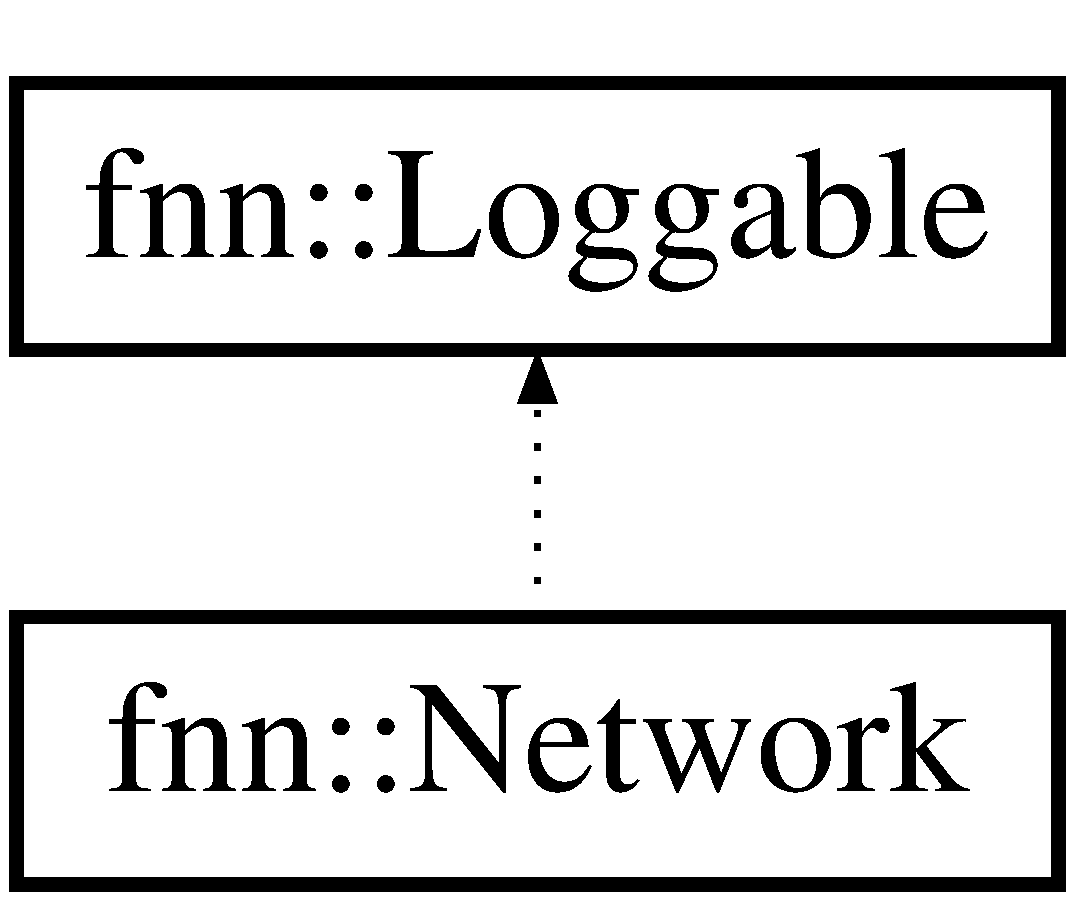
\includegraphics[height=2.000000cm]{classfnn_1_1_loggable}
\end{center}
\end{figure}
\subsection*{Public Member Functions}
\begin{DoxyCompactItemize}
\item 
\hyperlink{classfnn_1_1_loggable_a81f34c1fc8476ac4219c2ddb01c222d0}{Loggable} ()
\begin{DoxyCompactList}\small\item\em Default constructor. \end{DoxyCompactList}\item 
void \hyperlink{classfnn_1_1_loggable_a28a792b13dc2e4537bab2dbe7ff8a307}{Initialize} (\hyperlink{classfnn_1_1_log_manager}{Log\+Manager} $\ast$lm, string name, bool verbose)
\begin{DoxyCompactList}\small\item\em Constructs the logger. \end{DoxyCompactList}\item 
void \hyperlink{classfnn_1_1_loggable_a2e3828f6cf6e21652b12968bf44a78c5}{Log} (string log, string message, bool verbose=false)
\begin{DoxyCompactList}\small\item\em Logs a message to a specific log. \end{DoxyCompactList}\item 
void \hyperlink{classfnn_1_1_loggable_a117c6293cf156586db28af4c5d2515d1}{Add\+Log} (string name, bool verbose)
\begin{DoxyCompactList}\small\item\em Adds a log. \end{DoxyCompactList}\item 
void \hyperlink{classfnn_1_1_loggable_a01d0d53a2d3ae448050b0e1b1c159d65}{Set\+Verbose} (bool verbose)
\begin{DoxyCompactList}\small\item\em Sets a verbose. \end{DoxyCompactList}\item 
bool \hyperlink{classfnn_1_1_loggable_a6d86a105bbc849acbfc43955b224af06}{Is\+Verbose} ()
\begin{DoxyCompactList}\small\item\em Query if this object is verbose. \end{DoxyCompactList}\item 
std\+::vector$<$ \hyperlink{classfnn_1_1_log}{fnn\+::\+Log} $\ast$ $>$ \hyperlink{classfnn_1_1_loggable_ac067f3c5dcae780333636567844e0533}{Get\+Logs} ()
\begin{DoxyCompactList}\small\item\em Gets the logs. \end{DoxyCompactList}\item 
string \hyperlink{classfnn_1_1_loggable_a9b478a42733f406508f6ef47c4fffdf7}{Get\+Name} ()
\begin{DoxyCompactList}\small\item\em Gets the name. \end{DoxyCompactList}\end{DoxyCompactItemize}


\subsection{Detailed Description}
A loggable. 

=================================================================================================

\subsubsection*{William, 4/29/2015.  }

\subsection{Constructor \& Destructor Documentation}
\hypertarget{classfnn_1_1_loggable_a81f34c1fc8476ac4219c2ddb01c222d0}{}\index{fnn\+::\+Loggable@{fnn\+::\+Loggable}!Loggable@{Loggable}}
\index{Loggable@{Loggable}!fnn\+::\+Loggable@{fnn\+::\+Loggable}}
\subsubsection[{Loggable}]{\setlength{\rightskip}{0pt plus 5cm}fnn\+::\+Loggable\+::\+Loggable (
\begin{DoxyParamCaption}
\item[{void}]{}
\end{DoxyParamCaption}
)}\label{classfnn_1_1_loggable_a81f34c1fc8476ac4219c2ddb01c222d0}


Default constructor. 

=================================================================================================

\subsubsection*{William, 5/2/2015.  }

\subsection{Member Function Documentation}
\hypertarget{classfnn_1_1_loggable_a117c6293cf156586db28af4c5d2515d1}{}\index{fnn\+::\+Loggable@{fnn\+::\+Loggable}!Add\+Log@{Add\+Log}}
\index{Add\+Log@{Add\+Log}!fnn\+::\+Loggable@{fnn\+::\+Loggable}}
\subsubsection[{Add\+Log}]{\setlength{\rightskip}{0pt plus 5cm}void fnn\+::\+Loggable\+::\+Add\+Log (
\begin{DoxyParamCaption}
\item[{string}]{name, }
\item[{bool}]{verbose}
\end{DoxyParamCaption}
)}\label{classfnn_1_1_loggable_a117c6293cf156586db28af4c5d2515d1}


Adds a log. 

=================================================================================================

William, 4/29/2015. 

\subsubsection*{The name.  }\hypertarget{classfnn_1_1_loggable_ac067f3c5dcae780333636567844e0533}{}\index{fnn\+::\+Loggable@{fnn\+::\+Loggable}!Get\+Logs@{Get\+Logs}}
\index{Get\+Logs@{Get\+Logs}!fnn\+::\+Loggable@{fnn\+::\+Loggable}}
\subsubsection[{Get\+Logs}]{\setlength{\rightskip}{0pt plus 5cm}std\+::vector$<$ {\bf fnn\+::\+Log} $\ast$ $>$ fnn\+::\+Loggable\+::\+Get\+Logs (
\begin{DoxyParamCaption}
\item[{void}]{}
\end{DoxyParamCaption}
)}\label{classfnn_1_1_loggable_ac067f3c5dcae780333636567844e0533}


Gets the logs. 

=================================================================================================

William, 4/29/2015. 

\subsubsection*{null if it fails, else the logs.  }\hypertarget{classfnn_1_1_loggable_a9b478a42733f406508f6ef47c4fffdf7}{}\index{fnn\+::\+Loggable@{fnn\+::\+Loggable}!Get\+Name@{Get\+Name}}
\index{Get\+Name@{Get\+Name}!fnn\+::\+Loggable@{fnn\+::\+Loggable}}
\subsubsection[{Get\+Name}]{\setlength{\rightskip}{0pt plus 5cm}string fnn\+::\+Loggable\+::\+Get\+Name (
\begin{DoxyParamCaption}
\item[{void}]{}
\end{DoxyParamCaption}
)}\label{classfnn_1_1_loggable_a9b478a42733f406508f6ef47c4fffdf7}


Gets the name. 

=================================================================================================

William, 4/29/2015. 

\subsubsection*{The name.  }\hypertarget{classfnn_1_1_loggable_a28a792b13dc2e4537bab2dbe7ff8a307}{}\index{fnn\+::\+Loggable@{fnn\+::\+Loggable}!Initialize@{Initialize}}
\index{Initialize@{Initialize}!fnn\+::\+Loggable@{fnn\+::\+Loggable}}
\subsubsection[{Initialize}]{\setlength{\rightskip}{0pt plus 5cm}void fnn\+::\+Loggable\+::\+Initialize (
\begin{DoxyParamCaption}
\item[{{\bf Log\+Manager} $\ast$}]{lm, }
\item[{string}]{name, }
\item[{bool}]{verbose}
\end{DoxyParamCaption}
)}\label{classfnn_1_1_loggable_a28a792b13dc2e4537bab2dbe7ff8a307}


Constructs the logger. 

=================================================================================================

=================================================================================================

William, 4/29/2015. 


\begin{DoxyParams}{Parameters}
{\em lm} & \mbox{[}in,out\mbox{]} If non-\/null, the lm. \\
\hline
{\em name} & The name. \\
\hline
\end{DoxyParams}
\subsubsection*{true to verbose.  }

\subsection*{}

Constructs the logger. 

William, 4/29/2015. 

\subsubsection*{The name.  }

Initializes this object. 

William, 5/2/2015. 


\begin{DoxyParams}{Parameters}
{\em lm} & \mbox{[}in,out\mbox{]} If non-\/null, the lm. \\
\hline
{\em name} & The name. \\
\hline
\end{DoxyParams}
\subsubsection*{true to verbose.  }\hypertarget{classfnn_1_1_loggable_a6d86a105bbc849acbfc43955b224af06}{}\index{fnn\+::\+Loggable@{fnn\+::\+Loggable}!Is\+Verbose@{Is\+Verbose}}
\index{Is\+Verbose@{Is\+Verbose}!fnn\+::\+Loggable@{fnn\+::\+Loggable}}
\subsubsection[{Is\+Verbose}]{\setlength{\rightskip}{0pt plus 5cm}bool fnn\+::\+Loggable\+::\+Is\+Verbose (
\begin{DoxyParamCaption}
\item[{void}]{}
\end{DoxyParamCaption}
)}\label{classfnn_1_1_loggable_a6d86a105bbc849acbfc43955b224af06}


Query if this object is verbose. 

=================================================================================================

William, 4/29/2015. 

\subsubsection*{true if verbose, false if not.  }\hypertarget{classfnn_1_1_loggable_a2e3828f6cf6e21652b12968bf44a78c5}{}\index{fnn\+::\+Loggable@{fnn\+::\+Loggable}!Log@{Log}}
\index{Log@{Log}!fnn\+::\+Loggable@{fnn\+::\+Loggable}}
\subsubsection[{Log}]{\setlength{\rightskip}{0pt plus 5cm}void fnn\+::\+Loggable\+::\+Log (
\begin{DoxyParamCaption}
\item[{string}]{log, }
\item[{string}]{message, }
\item[{bool}]{verbose = {\ttfamily false}}
\end{DoxyParamCaption}
)}\label{classfnn_1_1_loggable_a2e3828f6cf6e21652b12968bf44a78c5}


Logs a message to a specific log. 

=================================================================================================

William, 4/29/2015. 


\begin{DoxyParams}{Parameters}
{\em log} & The log. \\
\hline
\end{DoxyParams}
\subsubsection*{The message.  }

=================================================================================================

William, 4/29/2015. 


\begin{DoxyParams}{Parameters}
{\em log} & The log. \\
\hline
{\em message} & The message. \\
\hline
\end{DoxyParams}
\subsubsection*{Whether or not (upon creation of a new log the log is verbose)  }\hypertarget{classfnn_1_1_loggable_a01d0d53a2d3ae448050b0e1b1c159d65}{}\index{fnn\+::\+Loggable@{fnn\+::\+Loggable}!Set\+Verbose@{Set\+Verbose}}
\index{Set\+Verbose@{Set\+Verbose}!fnn\+::\+Loggable@{fnn\+::\+Loggable}}
\subsubsection[{Set\+Verbose}]{\setlength{\rightskip}{0pt plus 5cm}void fnn\+::\+Loggable\+::\+Set\+Verbose (
\begin{DoxyParamCaption}
\item[{bool}]{verbose}
\end{DoxyParamCaption}
)}\label{classfnn_1_1_loggable_a01d0d53a2d3ae448050b0e1b1c159d65}


Sets a verbose. 

=================================================================================================

William, 4/29/2015. 

\subsubsection*{true to verbose.  }

The documentation for this class was generated from the following files\+:\begin{DoxyCompactItemize}
\item 
F\+N\+N++/\+F\+N\+N\+Lib/F\+N\+N\+Loggable.\+h\item 
F\+N\+N++/\+F\+N\+N\+Lib/F\+N\+N\+Loggable.\+cpp\end{DoxyCompactItemize}

\hypertarget{classfnn_1_1_log_manager}{}\section{fnn\+:\+:Log\+Manager Class Reference}
\label{classfnn_1_1_log_manager}\index{fnn\+::\+Log\+Manager@{fnn\+::\+Log\+Manager}}


Manager for logs.  




{\ttfamily \#include $<$F\+N\+N\+Log\+Manager.\+h$>$}

\subsection*{Public Member Functions}
\begin{DoxyCompactItemize}
\item 
\hyperlink{classfnn_1_1_log_manager_abb503c00777cd118edcf19bbb454b924}{Log\+Manager} ()
\begin{DoxyCompactList}\small\item\em Default constructor. \end{DoxyCompactList}\item 
void \hyperlink{classfnn_1_1_log_manager_a2af8bce7343fec5db9fe72443dbcdd65}{Register} (\hyperlink{classfnn_1_1_loggable}{Loggable} $\ast$logger, string logger\+Name, bool verbose)
\begin{DoxyCompactList}\small\item\em Registers a log with the \hyperlink{classfnn_1_1_log_manager}{Log\+Manager}. \end{DoxyCompactList}\item 
void \hyperlink{classfnn_1_1_log_manager_aee9f210a5a009e6f042656132ce67287}{Save} (string directory)
\begin{DoxyCompactList}\small\item\em Saves the set of all loggers under a directory and a sub directory. Consider is main logger property. \end{DoxyCompactList}\item 
void \hyperlink{classfnn_1_1_log_manager_a5f42cf3d05411c4d66202a823e3c6d55}{Print} (\hyperlink{classfnn_1_1_loggable}{Loggable} $\ast$logger, string log, string message)
\begin{DoxyCompactList}\small\item\em T\+O\+D\+O\+: Consider adding loading functionality. \end{DoxyCompactList}\end{DoxyCompactItemize}


\subsection{Detailed Description}
Manager for logs. 

=================================================================================================

\subsubsection*{William, 4/29/2015.  }

\subsection{Constructor \& Destructor Documentation}
\hypertarget{classfnn_1_1_log_manager_abb503c00777cd118edcf19bbb454b924}{}\index{fnn\+::\+Log\+Manager@{fnn\+::\+Log\+Manager}!Log\+Manager@{Log\+Manager}}
\index{Log\+Manager@{Log\+Manager}!fnn\+::\+Log\+Manager@{fnn\+::\+Log\+Manager}}
\subsubsection[{Log\+Manager}]{\setlength{\rightskip}{0pt plus 5cm}fnn\+::\+Log\+Manager\+::\+Log\+Manager (
\begin{DoxyParamCaption}
\item[{void}]{}
\end{DoxyParamCaption}
)}\label{classfnn_1_1_log_manager_abb503c00777cd118edcf19bbb454b924}


Default constructor. 

=================================================================================================

=================================================================================================

\subsubsection*{William, 4/29/2015.  }

\subsection*{}

Default constructor. 

\subsubsection*{William, 4/29/2015.  }

\subsection{Member Function Documentation}
\hypertarget{classfnn_1_1_log_manager_a5f42cf3d05411c4d66202a823e3c6d55}{}\index{fnn\+::\+Log\+Manager@{fnn\+::\+Log\+Manager}!Print@{Print}}
\index{Print@{Print}!fnn\+::\+Log\+Manager@{fnn\+::\+Log\+Manager}}
\subsubsection[{Print}]{\setlength{\rightskip}{0pt plus 5cm}void fnn\+::\+Log\+Manager\+::\+Print (
\begin{DoxyParamCaption}
\item[{{\bf Loggable} $\ast$}]{logger, }
\item[{string}]{log, }
\item[{string}]{message}
\end{DoxyParamCaption}
)}\label{classfnn_1_1_log_manager_a5f42cf3d05411c4d66202a823e3c6d55}


T\+O\+D\+O\+: Consider adding loading functionality. 

Prints a message to the verbose log. 

=================================================================================================

William, 5/3/2015. 


\begin{DoxyParams}{Parameters}
{\em logger} & \mbox{[}in,out\mbox{]} If non-\/null, the logger. \\
\hline
{\em log} & The log. \\
\hline
\end{DoxyParams}
\subsubsection*{The message.  }\hypertarget{classfnn_1_1_log_manager_a2af8bce7343fec5db9fe72443dbcdd65}{}\index{fnn\+::\+Log\+Manager@{fnn\+::\+Log\+Manager}!Register@{Register}}
\index{Register@{Register}!fnn\+::\+Log\+Manager@{fnn\+::\+Log\+Manager}}
\subsubsection[{Register}]{\setlength{\rightskip}{0pt plus 5cm}void fnn\+::\+Log\+Manager\+::\+Register (
\begin{DoxyParamCaption}
\item[{{\bf Loggable} $\ast$}]{logger, }
\item[{string}]{logger\+Name, }
\item[{bool}]{verbose}
\end{DoxyParamCaption}
)}\label{classfnn_1_1_log_manager_a2af8bce7343fec5db9fe72443dbcdd65}


Registers a log with the \hyperlink{classfnn_1_1_log_manager}{Log\+Manager}. 

=================================================================================================

William, 4/29/2015. 


\begin{DoxyParams}{Parameters}
{\em logger} & \mbox{[}in,out\mbox{]} The logger. \\
\hline
{\em logger\+Name} & Name of the logger. \\
\hline
\end{DoxyParams}
\subsubsection*{true to verbose.  }\hypertarget{classfnn_1_1_log_manager_aee9f210a5a009e6f042656132ce67287}{}\index{fnn\+::\+Log\+Manager@{fnn\+::\+Log\+Manager}!Save@{Save}}
\index{Save@{Save}!fnn\+::\+Log\+Manager@{fnn\+::\+Log\+Manager}}
\subsubsection[{Save}]{\setlength{\rightskip}{0pt plus 5cm}void fnn\+::\+Log\+Manager\+::\+Save (
\begin{DoxyParamCaption}
\item[{string}]{dir}
\end{DoxyParamCaption}
)}\label{classfnn_1_1_log_manager_aee9f210a5a009e6f042656132ce67287}


Saves the set of all loggers under a directory and a sub directory. Consider is main logger property. 

=================================================================================================

William, 4/29/2015. 

\subsubsection*{The directory to which to save.  }

=================================================================================================

William, 4/29/2015. 

\subsubsection*{The directory to which to save.  }

The documentation for this class was generated from the following files\+:\begin{DoxyCompactItemize}
\item 
F\+N\+N++/\+F\+N\+N\+Lib/F\+N\+N\+Log\+Manager.\+h\item 
F\+N\+N++/\+F\+N\+N\+Lib/F\+N\+N\+Log\+Manager.\+cpp\end{DoxyCompactItemize}

\hypertarget{classfnn_1_1_math}{}\section{fnn\+:\+:Math Class Reference}
\label{classfnn_1_1_math}\index{fnn\+::\+Math@{fnn\+::\+Math}}


The main mathematics helper class for F\+N\+N\+L\+I\+B  




{\ttfamily \#include $<$F\+N\+N\+Math.\+h$>$}

\subsection*{Static Public Member Functions}
\begin{DoxyCompactItemize}
\item 
static double \hyperlink{classfnn_1_1_math_a22635237c10b30c61d0eadc944f0bd29}{N\+Integrate} (std\+::function$<$ double(double)$>$ \&f, double a, double b, double eps)
\begin{DoxyCompactList}\small\item\em Numerically integrates any integrable function on a compact Hausdorff space. Integration occurs using Simpson\textquotesingle{}s rule. \end{DoxyCompactList}\item 
static double \hyperlink{classfnn_1_1_math_a2480fe29e114e12d9927b3f79ac6fc43}{N\+Integrate} (std\+::function$<$ double(double)$>$ \&f, double a, double b)
\begin{DoxyCompactList}\small\item\em Numerically integrates any integrable function using Simpson\textquotesingle{}s rule with auto scaling. \end{DoxyCompactList}\item 
static double \hyperlink{classfnn_1_1_math_a4e6ce151aa117f06b758fd37b76bb7de}{Uniform\+Real} (double min=0.\+0, double max=0.\+0)
\begin{DoxyCompactList}\small\item\em Uniform real. \end{DoxyCompactList}\item 
static double \hyperlink{classfnn_1_1_math_ad27de3d10960c2fd07ad68bccfffb192}{Gaussian\+Real} (double mean=0.\+0, double dev=1.\+0)
\begin{DoxyCompactList}\small\item\em Gaussian real. \end{DoxyCompactList}\item 
static std\+::vector$<$ double $>$ \hyperlink{classfnn_1_1_math_adad1b0610a61cf1f547902c63ac8f5f7}{Poly\+Mult} (std\+::vector$<$ double $>$ \&poly1, std\+::vector$<$ double $>$ \&poly2)
\begin{DoxyCompactList}\small\item\em A polynomial multiplication helper \end{DoxyCompactList}\item 
static std\+::function$<$ double(double)$>$ \hyperlink{classfnn_1_1_math_a14cd337326da37fa8e6943f868e5eace}{L\+E\+R\+P} (std\+::vector$<$ std\+::vector$<$ double $>$$>$ \&data)
\begin{DoxyCompactList}\small\item\em A linear interpolation algorithm \end{DoxyCompactList}\item 
static std\+::function$<$ double(double)$>$ \hyperlink{classfnn_1_1_math_a7f538718ad625d83a574b338a32d143e}{Lagrange\+Interpolation} (std\+::vector$<$ std\+::vector$<$ double $>$$>$ \&data)
\begin{DoxyCompactList}\small\item\em A polynomial interpolation algorithm using the Lagrange Interpolation Polynomial according to \href{http://en.wikipedia.org/wiki/Polynomial_interpolation}{\tt http\+://en.\+wikipedia.\+org/wiki/\+Polynomial\+\_\+interpolation} \end{DoxyCompactList}\item 
static int \hyperlink{classfnn_1_1_math_ad4998cc7ea2c63175d926eafedefd8c2}{Factorial} (int n)
\begin{DoxyCompactList}\small\item\em Factorial implementation. \end{DoxyCompactList}\item 
static std\+::vector$<$ double $>$ \hyperlink{classfnn_1_1_math_ac1d0f387a23294e585489c34dfccd2e4}{Gauss\+Jordan} (std\+::vector$<$ std\+::vector$<$ double $>$$>$ \&matrix)
\begin{DoxyCompactList}\small\item\em Gauss Jordan elimination for matrices. \end{DoxyCompactList}\item 
static std\+::function$<$ double(double)$>$ \hyperlink{classfnn_1_1_math_a6ae76ac184b97909719434da6081cc9c}{S\+Spline} (std\+::vector$<$ std\+::vector$<$ double $>$$>$ \&data)
\begin{DoxyCompactList}\small\item\em A simple spline interpolation algorithm as described in \href{http://www.geos.ed.ac.uk/~yliu23/docs/lect_spline.pdf}{\tt http\+://www.\+geos.\+ed.\+ac.\+uk/$\sim$yliu23/docs/lect\+\_\+spline.\+pdf}. Makes the assumption that the second derivative at the boundaries is equal to 0. \end{DoxyCompactList}\item 
static void \hyperlink{classfnn_1_1_math_a01efb86617a91478a89b94f83935234c}{Data\+Sort} (std\+::vector$<$ std\+::vector$<$ double $>$$>$ \&data)
\begin{DoxyCompactList}\small\item\em Data sort algorthim to sort by x-\/values of the data. Useful for the interpolation algorithms. \end{DoxyCompactList}\item 
static double \hyperlink{classfnn_1_1_math_ad08136c5ea2f35f1195d20781378ef76}{Mean} (std\+::vector$<$ double $>$ \&data)
\begin{DoxyCompactList}\small\item\em Determines the mean of the input vector. \end{DoxyCompactList}\item 
static double \hyperlink{classfnn_1_1_math_a51cadf575a006e30fcb43845a010f5bd}{Std\+Dev} (std\+::vector$<$ double $>$ \&data)
\begin{DoxyCompactList}\small\item\em Standard deviation of the data. \end{DoxyCompactList}\end{DoxyCompactItemize}


\subsection{Detailed Description}
The main mathematics helper class for F\+N\+N\+L\+I\+B 

=================================================================================================

\subsubsection*{William Guss, 4/6/2015.  }

\subsection{Member Function Documentation}
\hypertarget{classfnn_1_1_math_a01efb86617a91478a89b94f83935234c}{}\index{fnn\+::\+Math@{fnn\+::\+Math}!Data\+Sort@{Data\+Sort}}
\index{Data\+Sort@{Data\+Sort}!fnn\+::\+Math@{fnn\+::\+Math}}
\subsubsection[{Data\+Sort}]{\setlength{\rightskip}{0pt plus 5cm}void fnn\+::\+Math\+::\+Data\+Sort (
\begin{DoxyParamCaption}
\item[{std\+::vector$<$ std\+::vector$<$ double $>$$>$ \&}]{data}
\end{DoxyParamCaption}
)\hspace{0.3cm}{\ttfamily [static]}}\label{classfnn_1_1_math_a01efb86617a91478a89b94f83935234c}


Data sort algorthim to sort by x-\/values of the data. Useful for the interpolation algorithms. 

=================================================================================================

Phillip Kuznetsov, 4/29/2015. 


\begin{DoxyParams}{Parameters}
{\em data} & 2\+D vector of input data points. Each row is a point. \\
\hline
\end{DoxyParams}




=================================================================================================

Phillip Kuznetsov, 4/29/2015. 


\begin{DoxyParams}{Parameters}
{\em data} & 2\+D vector of input data points. Each row is a point. \\
\hline
\end{DoxyParams}


\subsubsection*{A 2\+D vector of the same points sorted.  }\hypertarget{classfnn_1_1_math_ad4998cc7ea2c63175d926eafedefd8c2}{}\index{fnn\+::\+Math@{fnn\+::\+Math}!Factorial@{Factorial}}
\index{Factorial@{Factorial}!fnn\+::\+Math@{fnn\+::\+Math}}
\subsubsection[{Factorial}]{\setlength{\rightskip}{0pt plus 5cm}int fnn\+::\+Math\+::\+Factorial (
\begin{DoxyParamCaption}
\item[{int}]{n}
\end{DoxyParamCaption}
)\hspace{0.3cm}{\ttfamily [static]}}\label{classfnn_1_1_math_ad4998cc7ea2c63175d926eafedefd8c2}


Factorial implementation. 

=================================================================================================

William, 4/26/2015. 


\begin{DoxyParams}{Parameters}
{\em n} & The int to process. \\
\hline
\end{DoxyParams}


\subsubsection*{An int.  }\hypertarget{classfnn_1_1_math_ad27de3d10960c2fd07ad68bccfffb192}{}\index{fnn\+::\+Math@{fnn\+::\+Math}!Gaussian\+Real@{Gaussian\+Real}}
\index{Gaussian\+Real@{Gaussian\+Real}!fnn\+::\+Math@{fnn\+::\+Math}}
\subsubsection[{Gaussian\+Real}]{\setlength{\rightskip}{0pt plus 5cm}double fnn\+::\+Math\+::\+Gaussian\+Real (
\begin{DoxyParamCaption}
\item[{double}]{mean = {\ttfamily 0.0}, }
\item[{double}]{dev = {\ttfamily 1.0}}
\end{DoxyParamCaption}
)\hspace{0.3cm}{\ttfamily [static]}}\label{classfnn_1_1_math_ad27de3d10960c2fd07ad68bccfffb192}


Gaussian real. 

=================================================================================================

William Guss, 4/11/2015. 


\begin{DoxyParams}{Parameters}
{\em mean} & The mean. \\
\hline
\end{DoxyParams}


\subsubsection*{A double.  }\hypertarget{classfnn_1_1_math_ac1d0f387a23294e585489c34dfccd2e4}{}\index{fnn\+::\+Math@{fnn\+::\+Math}!Gauss\+Jordan@{Gauss\+Jordan}}
\index{Gauss\+Jordan@{Gauss\+Jordan}!fnn\+::\+Math@{fnn\+::\+Math}}
\subsubsection[{Gauss\+Jordan}]{\setlength{\rightskip}{0pt plus 5cm}std\+::vector$<$ double $>$ fnn\+::\+Math\+::\+Gauss\+Jordan (
\begin{DoxyParamCaption}
\item[{std\+::vector$<$ std\+::vector$<$ double $>$$>$ \&}]{matrix}
\end{DoxyParamCaption}
)\hspace{0.3cm}{\ttfamily [static]}}\label{classfnn_1_1_math_ac1d0f387a23294e585489c34dfccd2e4}


Gauss Jordan elimination for matrices. 

=================================================================================================

Phillip Kuznetsov, 4/29/2015. 


\begin{DoxyParams}{Parameters}
{\em matrix} & The systems of equation augmented matrix. \\
\hline
\end{DoxyParams}


\subsubsection*{A vector of the variable values solved by completed Gauss-\/\+Jordan elimination.  }

=================================================================================================

Phillip Kuznetsov, 4/29/2015. 


\begin{DoxyParams}{Parameters}
{\em matrix} & The systems of equation augmented matrix. Passes by reference. \\
\hline
\end{DoxyParams}


\subsubsection*{A vector of the variable values solved by completed Gauss-\/\+Jordan elimination.  }\hypertarget{classfnn_1_1_math_a7f538718ad625d83a574b338a32d143e}{}\index{fnn\+::\+Math@{fnn\+::\+Math}!Lagrange\+Interpolation@{Lagrange\+Interpolation}}
\index{Lagrange\+Interpolation@{Lagrange\+Interpolation}!fnn\+::\+Math@{fnn\+::\+Math}}
\subsubsection[{Lagrange\+Interpolation}]{\setlength{\rightskip}{0pt plus 5cm}std\+::function$<$ double(double)$>$ fnn\+::\+Math\+::\+Lagrange\+Interpolation (
\begin{DoxyParamCaption}
\item[{std\+::vector$<$ std\+::vector$<$ double $>$$>$ \&}]{data}
\end{DoxyParamCaption}
)\hspace{0.3cm}{\ttfamily [static]}}\label{classfnn_1_1_math_a7f538718ad625d83a574b338a32d143e}


A polynomial interpolation algorithm using the Lagrange Interpolation Polynomial according to \href{http://en.wikipedia.org/wiki/Polynomial_interpolation}{\tt http\+://en.\+wikipedia.\+org/wiki/\+Polynomial\+\_\+interpolation} 

=================================================================================================

Phillip Kuznetsov, 4/19/2015. 


\begin{DoxyParams}{Parameters}
{\em data} & 2\+D vector of input data points. Each row is a point. \\
\hline
\end{DoxyParams}


\subsubsection*{A polynomial interpolation function  }\hypertarget{classfnn_1_1_math_a14cd337326da37fa8e6943f868e5eace}{}\index{fnn\+::\+Math@{fnn\+::\+Math}!L\+E\+R\+P@{L\+E\+R\+P}}
\index{L\+E\+R\+P@{L\+E\+R\+P}!fnn\+::\+Math@{fnn\+::\+Math}}
\subsubsection[{L\+E\+R\+P}]{\setlength{\rightskip}{0pt plus 5cm}std\+::function$<$ double(double)$>$ fnn\+::\+Math\+::\+L\+E\+R\+P (
\begin{DoxyParamCaption}
\item[{std\+::vector$<$ std\+::vector$<$ double $>$$>$ \&}]{data}
\end{DoxyParamCaption}
)\hspace{0.3cm}{\ttfamily [static]}}\label{classfnn_1_1_math_a14cd337326da37fa8e6943f868e5eace}


A linear interpolation algorithm 

=================================================================================================

Phillip Kuznetsov, 4/18/2015. 


\begin{DoxyParams}{Parameters}
{\em data} & 2\+D vector of input data points \\
\hline
\end{DoxyParams}


\subsubsection*{A linear interpolation function  }\hypertarget{classfnn_1_1_math_ad08136c5ea2f35f1195d20781378ef76}{}\index{fnn\+::\+Math@{fnn\+::\+Math}!Mean@{Mean}}
\index{Mean@{Mean}!fnn\+::\+Math@{fnn\+::\+Math}}
\subsubsection[{Mean}]{\setlength{\rightskip}{0pt plus 5cm}double fnn\+::\+Math\+::\+Mean (
\begin{DoxyParamCaption}
\item[{std\+::vector$<$ double $>$ \&}]{data}
\end{DoxyParamCaption}
)\hspace{0.3cm}{\ttfamily [static]}}\label{classfnn_1_1_math_ad08136c5ea2f35f1195d20781378ef76}


Determines the mean of the input vector. 

Phillip Kuznetsov, 5/6/2015. 


\begin{DoxyParams}{Parameters}
{\em data} & The data. \\
\hline
\end{DoxyParams}


\begin{DoxyReturn}{Returns}
The mean of the data 
\end{DoxyReturn}


Phillip Kuznetsov, 5/6/2015. 


\begin{DoxyParams}{Parameters}
{\em data} & The data. \\
\hline
\end{DoxyParams}


\begin{DoxyReturn}{Returns}
The mean of the data. 
\end{DoxyReturn}
\hypertarget{classfnn_1_1_math_a22635237c10b30c61d0eadc944f0bd29}{}\index{fnn\+::\+Math@{fnn\+::\+Math}!N\+Integrate@{N\+Integrate}}
\index{N\+Integrate@{N\+Integrate}!fnn\+::\+Math@{fnn\+::\+Math}}
\subsubsection[{N\+Integrate}]{\setlength{\rightskip}{0pt plus 5cm}double fnn\+::\+Math\+::\+N\+Integrate (
\begin{DoxyParamCaption}
\item[{std\+::function$<$ double(double)$>$ \&}]{f, }
\item[{double}]{a, }
\item[{double}]{b, }
\item[{double}]{eps}
\end{DoxyParamCaption}
)\hspace{0.3cm}{\ttfamily [static]}}\label{classfnn_1_1_math_a22635237c10b30c61d0eadc944f0bd29}


Numerically integrates any integrable function on a compact Hausdorff space. Integration occurs using Simpson\textquotesingle{}s rule. 

=================================================================================================

William Guss, 4/6/2015. 


\begin{DoxyParams}{Parameters}
{\em f} & The function to integrate. \\
\hline
{\em a} & The lower bound of integration. \\
\hline
{\em b} & The upper bound of integration. \\
\hline
{\em eps} & The step-\/size of integration using Simpson\textquotesingle{}s rule.\\
\hline
\end{DoxyParams}


\subsubsection*{The result.  }

=================================================================================================

William Guss, 4/6/2015. 


\begin{DoxyParams}{Parameters}
{\em f} & The function to integrate. \\
\hline
{\em a} & The lower bound of integration. \\
\hline
{\em b} & The upper bound of integration. \\
\hline
{\em eps} & The step-\/size of integration using Simpson\textquotesingle{}s rule. \\
\hline
\end{DoxyParams}


\subsubsection*{The result.  }\hypertarget{classfnn_1_1_math_a2480fe29e114e12d9927b3f79ac6fc43}{}\index{fnn\+::\+Math@{fnn\+::\+Math}!N\+Integrate@{N\+Integrate}}
\index{N\+Integrate@{N\+Integrate}!fnn\+::\+Math@{fnn\+::\+Math}}
\subsubsection[{N\+Integrate}]{\setlength{\rightskip}{0pt plus 5cm}double fnn\+::\+Math\+::\+N\+Integrate (
\begin{DoxyParamCaption}
\item[{std\+::function$<$ double(double)$>$ \&}]{f, }
\item[{double}]{a, }
\item[{double}]{b}
\end{DoxyParamCaption}
)\hspace{0.3cm}{\ttfamily [static]}}\label{classfnn_1_1_math_a2480fe29e114e12d9927b3f79ac6fc43}


Numerically integrates any integrable function using Simpson\textquotesingle{}s rule with auto scaling. 

=================================================================================================

William Guss, 4/6/2015. 


\begin{DoxyParams}{Parameters}
{\em f} & The function to integrate. \\
\hline
{\em a} & The lower bound of integration. \\
\hline
{\em b} & The upper bound of integration. \\
\hline
\end{DoxyParams}


\subsubsection*{The result.  }\hypertarget{classfnn_1_1_math_adad1b0610a61cf1f547902c63ac8f5f7}{}\index{fnn\+::\+Math@{fnn\+::\+Math}!Poly\+Mult@{Poly\+Mult}}
\index{Poly\+Mult@{Poly\+Mult}!fnn\+::\+Math@{fnn\+::\+Math}}
\subsubsection[{Poly\+Mult}]{\setlength{\rightskip}{0pt plus 5cm}std\+::vector$<$ double $>$ fnn\+::\+Math\+::\+Poly\+Mult (
\begin{DoxyParamCaption}
\item[{std\+::vector$<$ double $>$ \&}]{poly1, }
\item[{std\+::vector$<$ double $>$ \&}]{poly2}
\end{DoxyParamCaption}
)\hspace{0.3cm}{\ttfamily [static]}}\label{classfnn_1_1_math_adad1b0610a61cf1f547902c63ac8f5f7}


A polynomial multiplication helper 

=================================================================================================

Phillip Kuznetsov, 4/19/2015. 


\begin{DoxyParams}{Parameters}
{\em poly1} & A vector of the coefficients. Each index is the power which x is raised to\\
\hline
\end{DoxyParams}



\begin{DoxyParams}{Parameters}
{\em poly2} & A vector of the second polynomial coefficients./param$>$\\
\hline
\end{DoxyParams}
\subsubsection*{A vector of coefficients for hte polynomial  }\hypertarget{classfnn_1_1_math_a6ae76ac184b97909719434da6081cc9c}{}\index{fnn\+::\+Math@{fnn\+::\+Math}!S\+Spline@{S\+Spline}}
\index{S\+Spline@{S\+Spline}!fnn\+::\+Math@{fnn\+::\+Math}}
\subsubsection[{S\+Spline}]{\setlength{\rightskip}{0pt plus 5cm}std\+::function$<$ double(double)$>$ fnn\+::\+Math\+::\+S\+Spline (
\begin{DoxyParamCaption}
\item[{std\+::vector$<$ std\+::vector$<$ double $>$$>$ \&}]{data}
\end{DoxyParamCaption}
)\hspace{0.3cm}{\ttfamily [static]}}\label{classfnn_1_1_math_a6ae76ac184b97909719434da6081cc9c}


A simple spline interpolation algorithm as described in \href{http://www.geos.ed.ac.uk/~yliu23/docs/lect_spline.pdf}{\tt http\+://www.\+geos.\+ed.\+ac.\+uk/$\sim$yliu23/docs/lect\+\_\+spline.\+pdf}. Makes the assumption that the second derivative at the boundaries is equal to 0. 

=================================================================================================

Phillip Kuznetsov, 4/29/2015. 


\begin{DoxyParams}{Parameters}
{\em data} & 2\+D vector of input data points. Each row is a point. \\
\hline
\end{DoxyParams}


\subsubsection*{A polynomial interpolation function  }

=================================================================================================

Phillip Kuznetsov, 4/29/2015. 

\subsubsection*{2\+D vector of input data points. Each row is a point.  }k\+: the vector of three coordinates that the current spline is working with. Dimensions are (x,y)

The coefficents of the equation d$^\wedge$2f(k-\/1)/dx$^\wedge$2 coef\mbox{[}0\mbox{]} +d$^\wedge$2f(k)/dx$^\wedge$2 coef\mbox{[}1\mbox{]} +d$^\wedge$2f(k+1)/dx$^\wedge$2 coef\mbox{[}2\mbox{]} 

The coefs index counter. The for loop goes through the row and fills them with the three coefficients of the equation set. 

This is why we initialized the size to data.\+size()+1. \hypertarget{classfnn_1_1_math_a51cadf575a006e30fcb43845a010f5bd}{}\index{fnn\+::\+Math@{fnn\+::\+Math}!Std\+Dev@{Std\+Dev}}
\index{Std\+Dev@{Std\+Dev}!fnn\+::\+Math@{fnn\+::\+Math}}
\subsubsection[{Std\+Dev}]{\setlength{\rightskip}{0pt plus 5cm}double fnn\+::\+Math\+::\+Std\+Dev (
\begin{DoxyParamCaption}
\item[{std\+::vector$<$ double $>$ \&}]{data}
\end{DoxyParamCaption}
)\hspace{0.3cm}{\ttfamily [static]}}\label{classfnn_1_1_math_a51cadf575a006e30fcb43845a010f5bd}


Standard deviation of the data. 

The population standard deviation of the data. 

Phillip Kuznetsov, 5/6/2015. 


\begin{DoxyParams}{Parameters}
{\em data} & The data. \\
\hline
\end{DoxyParams}


\begin{DoxyReturn}{Returns}
The standard deviation of the data 
\end{DoxyReturn}


Phillip Kuznetsov, 5/6/2015. 


\begin{DoxyParams}{Parameters}
{\em data} & The data. \\
\hline
\end{DoxyParams}


\begin{DoxyReturn}{Returns}
The standard deviation of the data. 
\end{DoxyReturn}
\hypertarget{classfnn_1_1_math_a4e6ce151aa117f06b758fd37b76bb7de}{}\index{fnn\+::\+Math@{fnn\+::\+Math}!Uniform\+Real@{Uniform\+Real}}
\index{Uniform\+Real@{Uniform\+Real}!fnn\+::\+Math@{fnn\+::\+Math}}
\subsubsection[{Uniform\+Real}]{\setlength{\rightskip}{0pt plus 5cm}double fnn\+::\+Math\+::\+Uniform\+Real (
\begin{DoxyParamCaption}
\item[{double}]{min = {\ttfamily 0.0}, }
\item[{double}]{max = {\ttfamily 0.0}}
\end{DoxyParamCaption}
)\hspace{0.3cm}{\ttfamily [static]}}\label{classfnn_1_1_math_a4e6ce151aa117f06b758fd37b76bb7de}


Uniform real. 

=================================================================================================

William Guss, 4/11/2015. 


\begin{DoxyParams}{Parameters}
{\em min} & The minimum. \\
\hline
{\em max} & The maximum. \\
\hline
\end{DoxyParams}


\subsubsection*{A double.  }

The documentation for this class was generated from the following files\+:\begin{DoxyCompactItemize}
\item 
F\+N\+N++/\+F\+N\+N\+Lib/F\+N\+N\+Math.\+h\item 
F\+N\+N++/\+F\+N\+N\+Lib/F\+N\+N\+Math.\+cpp\end{DoxyCompactItemize}

\hypertarget{classfnn_1_1_network}{}\section{fnn\+:\+:Network Class Reference}
\label{classfnn_1_1_network}\index{fnn\+::\+Network@{fnn\+::\+Network}}


The main class of operation on the functional neural networks.  




{\ttfamily \#include $<$F\+N\+N\+Network.\+h$>$}

Inheritance diagram for fnn\+:\+:Network\+:\begin{figure}[H]
\begin{center}
\leavevmode
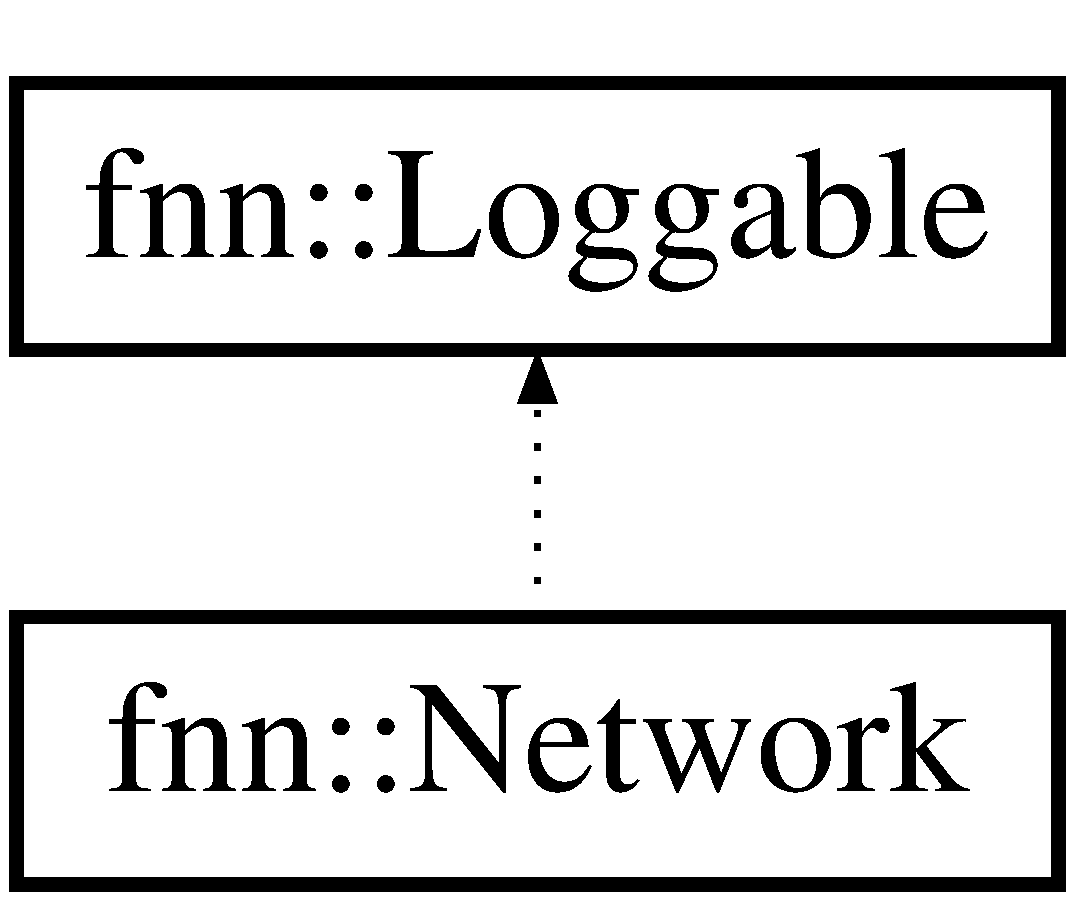
\includegraphics[height=2.000000cm]{classfnn_1_1_network}
\end{center}
\end{figure}
\subsection*{Public Member Functions}
\begin{DoxyCompactItemize}
\item 
\hyperlink{classfnn_1_1_network_a5dd4695e1ce543dafc188d86cd691465}{Network} ()
\begin{DoxyCompactList}\small\item\em Constructs a functional neural network.. \end{DoxyCompactList}\item 
std\+::function$<$ double(double)$>$ \hyperlink{classfnn_1_1_network_a9e3f194d0b23fbdd92873b202798e1f9}{Feed\+Forward} (std\+::function$<$ double(double)$>$ ξ)
\begin{DoxyCompactList}\small\item\em Runs the network using the fast feedforward algorithm. The algorithm caches following that described in the paper. \end{DoxyCompactList}\item 
double \hyperlink{classfnn_1_1_network_a46144de037977a237b058db79bdb5cad}{Back\+Propagate} (std\+::function$<$ double(double)$>$ δ)
\begin{DoxyCompactList}\small\item\em Back propagate using the Super Pro Algo developed by William Guss and Patrick Chen. \end{DoxyCompactList}\item 
void \hyperlink{classfnn_1_1_network_a16e2878c6cc2dcb053c8c9ead48cd021}{Set\+Activation} (\hyperlink{classfnn_1_1_sigmoid}{Sigmoid} activator)
\begin{DoxyCompactList}\small\item\em Sets an activation. \end{DoxyCompactList}\item 
void \hyperlink{classfnn_1_1_network_a96ecfd11618f4abb26df9495bb904725}{Add\+Layer} (int x, int y)
\begin{DoxyCompactList}\small\item\em Adds a layer to \textquotesingle{}y\textquotesingle{}. \end{DoxyCompactList}\item 
double \hyperlink{classfnn_1_1_network_a38ed0637972cb29a3a0bc2b55a52979a}{Train} (\hyperlink{structfnn_1_1_data_point}{Data\+Point} \&dp, std\+::vector$<$ double $>$ learning\+Parameters)
\begin{DoxyCompactList}\small\item\em Trains the network \end{DoxyCompactList}\item 
void \hyperlink{classfnn_1_1_network_a8d794dcaf3949c7363950b61f572b78b}{Nudge\+Weights} ()
\begin{DoxyCompactList}\small\item\em Nudge weights. \end{DoxyCompactList}\end{DoxyCompactItemize}
\subsection*{Public Attributes}
\begin{DoxyCompactItemize}
\item 
\hyperlink{classfnn_1_1_sigmoid}{Sigmoid} \hyperlink{classfnn_1_1_network_a28a1473ecd20a30d85e4a256dc2cf12a}{Activator}
\begin{DoxyCompactList}\small\item\em The primary activator type for the neural network. \end{DoxyCompactList}\end{DoxyCompactItemize}


\subsection{Detailed Description}
The main class of operation on the functional neural networks. 

=================================================================================================

\subsubsection*{William, 4/9/2015.  }

\subsection{Constructor \& Destructor Documentation}
\hypertarget{classfnn_1_1_network_a5dd4695e1ce543dafc188d86cd691465}{}\index{fnn\+::\+Network@{fnn\+::\+Network}!Network@{Network}}
\index{Network@{Network}!fnn\+::\+Network@{fnn\+::\+Network}}
\subsubsection[{Network}]{\setlength{\rightskip}{0pt plus 5cm}fnn\+::\+Network\+::\+Network (
\begin{DoxyParamCaption}
{}
\end{DoxyParamCaption}
)}\label{classfnn_1_1_network_a5dd4695e1ce543dafc188d86cd691465}


Constructs a functional neural network.. 

=================================================================================================

=================================================================================================

William, 4/10/2015. 

\subsubsection*{The layer count.  }

\subsection*{}

Constructs a functional neural network. 

William, 4/10/2015. 

\subsubsection*{The layer count.  }

\subsection{Member Function Documentation}
\hypertarget{classfnn_1_1_network_a96ecfd11618f4abb26df9495bb904725}{}\index{fnn\+::\+Network@{fnn\+::\+Network}!Add\+Layer@{Add\+Layer}}
\index{Add\+Layer@{Add\+Layer}!fnn\+::\+Network@{fnn\+::\+Network}}
\subsubsection[{Add\+Layer}]{\setlength{\rightskip}{0pt plus 5cm}void fnn\+::\+Network\+::\+Add\+Layer (
\begin{DoxyParamCaption}
\item[{int}]{x, }
\item[{int}]{y}
\end{DoxyParamCaption}
)}\label{classfnn_1_1_network_a96ecfd11618f4abb26df9495bb904725}


Adds a layer to \textquotesingle{}y\textquotesingle{}. 

=================================================================================================

William Guss, 4/12/2015. 


\begin{DoxyParams}{Parameters}
{\em x} & The x coordinate. \\
\hline
\end{DoxyParams}
\subsubsection*{The y coordinate.  }\hypertarget{classfnn_1_1_network_a46144de037977a237b058db79bdb5cad}{}\index{fnn\+::\+Network@{fnn\+::\+Network}!Back\+Propagate@{Back\+Propagate}}
\index{Back\+Propagate@{Back\+Propagate}!fnn\+::\+Network@{fnn\+::\+Network}}
\subsubsection[{Back\+Propagate}]{\setlength{\rightskip}{0pt plus 5cm}double fnn\+::\+Network\+::\+Back\+Propagate (
\begin{DoxyParamCaption}
\item[{std\+::function$<$ double(double)$>$}]{δ}
\end{DoxyParamCaption}
)}\label{classfnn_1_1_network_a46144de037977a237b058db79bdb5cad}


Back propagate using the Super Pro Algo developed by William Guss and Patrick Chen. 

=================================================================================================

William Guss, 5/6/2015. 


\begin{DoxyParams}{Parameters}
{\em δ} & The desired function delta δ. \\
\hline
\end{DoxyParams}


\subsubsection*{The total integrated error over the last interval.  }\hypertarget{classfnn_1_1_network_a9e3f194d0b23fbdd92873b202798e1f9}{}\index{fnn\+::\+Network@{fnn\+::\+Network}!Feed\+Forward@{Feed\+Forward}}
\index{Feed\+Forward@{Feed\+Forward}!fnn\+::\+Network@{fnn\+::\+Network}}
\subsubsection[{Feed\+Forward}]{\setlength{\rightskip}{0pt plus 5cm}std\+::function$<$ double(double)$>$ fnn\+::\+Network\+::\+Feed\+Forward (
\begin{DoxyParamCaption}
\item[{std\+::function$<$ double(double)$>$}]{ξ}
\end{DoxyParamCaption}
)}\label{classfnn_1_1_network_a9e3f194d0b23fbdd92873b202798e1f9}


Runs the network using the fast feedforward algorithm. The algorithm caches following that described in the paper. 

=================================================================================================

William, 4/10/2015. 


\begin{DoxyParams}{Parameters}
{\em ξ} & The input, ξ. \\
\hline
\end{DoxyParams}


\subsubsection*{The ouput, F\mbox{[}ξ\mbox{]}.  }\hypertarget{classfnn_1_1_network_a8d794dcaf3949c7363950b61f572b78b}{}\index{fnn\+::\+Network@{fnn\+::\+Network}!Nudge\+Weights@{Nudge\+Weights}}
\index{Nudge\+Weights@{Nudge\+Weights}!fnn\+::\+Network@{fnn\+::\+Network}}
\subsubsection[{Nudge\+Weights}]{\setlength{\rightskip}{0pt plus 5cm}void fnn\+::\+Network\+::\+Nudge\+Weights (
\begin{DoxyParamCaption}
\item[{void}]{}
\end{DoxyParamCaption}
)}\label{classfnn_1_1_network_a8d794dcaf3949c7363950b61f572b78b}


Nudge weights. 

Phillip Kuznetsov, 5/8/2015. \hypertarget{classfnn_1_1_network_a16e2878c6cc2dcb053c8c9ead48cd021}{}\index{fnn\+::\+Network@{fnn\+::\+Network}!Set\+Activation@{Set\+Activation}}
\index{Set\+Activation@{Set\+Activation}!fnn\+::\+Network@{fnn\+::\+Network}}
\subsubsection[{Set\+Activation}]{\setlength{\rightskip}{0pt plus 5cm}void fnn\+::\+Network\+::\+Set\+Activation (
\begin{DoxyParamCaption}
\item[{{\bf Sigmoid}}]{activator}
\end{DoxyParamCaption}
)}\label{classfnn_1_1_network_a16e2878c6cc2dcb053c8c9ead48cd021}


Sets an activation. 

=================================================================================================

William Guss, 4/11/2015. 

\subsubsection*{The activator.  }\hypertarget{classfnn_1_1_network_a38ed0637972cb29a3a0bc2b55a52979a}{}\index{fnn\+::\+Network@{fnn\+::\+Network}!Train@{Train}}
\index{Train@{Train}!fnn\+::\+Network@{fnn\+::\+Network}}
\subsubsection[{Train}]{\setlength{\rightskip}{0pt plus 5cm}double fnn\+::\+Network\+::\+Train (
\begin{DoxyParamCaption}
\item[{{\bf Data\+Point} \&}]{dp, }
\item[{std\+::vector$<$ double $>$}]{learning\+Parameters}
\end{DoxyParamCaption}
)}\label{classfnn_1_1_network_a38ed0637972cb29a3a0bc2b55a52979a}


Trains the network 

Trains the network. 

Phillip Kuznetsov, 5/8/2015. 


\begin{DoxyParams}{Parameters}
{\em ds} & The current datapoint \\
\hline
{\em learning\+Parameters} & Options for controlling the learning. \\
\hline
\end{DoxyParams}


\begin{DoxyReturn}{Returns}
A double. 
\end{DoxyReturn}


Phillip Kuznetsov, 5/8/2015. 


\begin{DoxyParams}{Parameters}
{\em dp} & The current datapoint. \\
\hline
{\em learning\+Parameters} & Options for controlling the learning. \\
\hline
\end{DoxyParams}


\begin{DoxyReturn}{Returns}
A double. 
\end{DoxyReturn}


\subsection{Member Data Documentation}
\hypertarget{classfnn_1_1_network_a28a1473ecd20a30d85e4a256dc2cf12a}{}\index{fnn\+::\+Network@{fnn\+::\+Network}!Activator@{Activator}}
\index{Activator@{Activator}!fnn\+::\+Network@{fnn\+::\+Network}}
\subsubsection[{Activator}]{\setlength{\rightskip}{0pt plus 5cm}{\bf Sigmoid} fnn\+::\+Network\+::\+Activator}\label{classfnn_1_1_network_a28a1473ecd20a30d85e4a256dc2cf12a}


The primary activator type for the neural network. 



The documentation for this class was generated from the following files\+:\begin{DoxyCompactItemize}
\item 
F\+N\+N++/\+F\+N\+N\+Lib/F\+N\+N\+Network.\+h\item 
F\+N\+N++/\+F\+N\+N\+Lib/F\+N\+N\+Network.\+cpp\end{DoxyCompactItemize}

\hypertarget{classfnn_1_1_sigmoid}{}\section{fnn\+:\+:Sigmoid Class Reference}
\label{classfnn_1_1_sigmoid}\index{fnn\+::\+Sigmoid@{fnn\+::\+Sigmoid}}
\subsection*{Public Member Functions}
\begin{DoxyCompactItemize}
\item 
\hyperlink{classfnn_1_1_sigmoid_a3ea6f3057765aaf64000c87601b4dedb}{Sigmoid} (std\+::function$<$ double(double)$>$ f, std\+::function$<$ double(double)$>$ fprime)
\begin{DoxyCompactList}\small\item\em Constructs a sigmoid function \end{DoxyCompactList}\item 
\hyperlink{classfnn_1_1_sigmoid_a67b28b32d36e6e831051677234b0e2a4}{Sigmoid} ()
\begin{DoxyCompactList}\small\item\em Default constructor. \end{DoxyCompactList}\item 
double \hyperlink{classfnn_1_1_sigmoid_a90bd1a37bd4ad4f5a4074f364430b85d}{prime} (double x)
\begin{DoxyCompactList}\small\item\em Evaluates the derivative of the activation function. \end{DoxyCompactList}\item 
double \hyperlink{classfnn_1_1_sigmoid_afc3a732e3ab0e5b00601564d4e220283}{operator()} (double x)
\begin{DoxyCompactList}\small\item\em Evaluates the sigmoid. \end{DoxyCompactList}\end{DoxyCompactItemize}
\subsection*{Static Public Member Functions}
\begin{DoxyCompactItemize}
\item 
static \hyperlink{classfnn_1_1_sigmoid}{Sigmoid} \hyperlink{classfnn_1_1_sigmoid_a15cba16e03aeb3bca3429640e513bbc8}{Linear} ()
\begin{DoxyCompactList}\small\item\em Gets the linear sigmoid activation. \end{DoxyCompactList}\item 
static \hyperlink{classfnn_1_1_sigmoid}{Sigmoid} \hyperlink{classfnn_1_1_sigmoid_a67434428fa6cc846ea4c7cb9a5d04983}{Logistic} ()
\begin{DoxyCompactList}\small\item\em The logistic activation function. \end{DoxyCompactList}\item 
static \hyperlink{classfnn_1_1_sigmoid}{Sigmoid} \hyperlink{classfnn_1_1_sigmoid_a616038ee95650af8b0a14c8b5ee20799}{Tanh} ()
\begin{DoxyCompactList}\small\item\em Gets the hyperbolic tangent activation function. \end{DoxyCompactList}\end{DoxyCompactItemize}


\subsection{Constructor \& Destructor Documentation}
\hypertarget{classfnn_1_1_sigmoid_a3ea6f3057765aaf64000c87601b4dedb}{}\index{fnn\+::\+Sigmoid@{fnn\+::\+Sigmoid}!Sigmoid@{Sigmoid}}
\index{Sigmoid@{Sigmoid}!fnn\+::\+Sigmoid@{fnn\+::\+Sigmoid}}
\subsubsection[{Sigmoid}]{\setlength{\rightskip}{0pt plus 5cm}fnn\+::\+Sigmoid\+::\+Sigmoid (
\begin{DoxyParamCaption}
\item[{std\+::function$<$ double(double)$>$}]{g, }
\item[{std\+::function$<$ double(double)$>$}]{gprime}
\end{DoxyParamCaption}
)}\label{classfnn_1_1_sigmoid_a3ea6f3057765aaf64000c87601b4dedb}


Constructs a sigmoid function 

Default constructor. Do nothing.\+t 

=================================================================================================

William, 4/10/2015. 


\begin{DoxyParams}{Parameters}
{\em f} & The std\+::function$<$double(double)$>$ to process. \\
\hline
\end{DoxyParams}
\subsubsection*{The fprime.  }

=================================================================================================

\subsubsection*{William Guss, 4/12/2015.  }\hypertarget{classfnn_1_1_sigmoid_a67b28b32d36e6e831051677234b0e2a4}{}\index{fnn\+::\+Sigmoid@{fnn\+::\+Sigmoid}!Sigmoid@{Sigmoid}}
\index{Sigmoid@{Sigmoid}!fnn\+::\+Sigmoid@{fnn\+::\+Sigmoid}}
\subsubsection[{Sigmoid}]{\setlength{\rightskip}{0pt plus 5cm}fnn\+::\+Sigmoid\+::\+Sigmoid (
\begin{DoxyParamCaption}
{}
\end{DoxyParamCaption}
)}\label{classfnn_1_1_sigmoid_a67b28b32d36e6e831051677234b0e2a4}


Default constructor. 

Default constructor. Do nothing.\+t 

=================================================================================================

\subsubsection*{William Guss, 4/12/2015.  }

\subsection{Member Function Documentation}
\hypertarget{classfnn_1_1_sigmoid_a15cba16e03aeb3bca3429640e513bbc8}{}\index{fnn\+::\+Sigmoid@{fnn\+::\+Sigmoid}!Linear@{Linear}}
\index{Linear@{Linear}!fnn\+::\+Sigmoid@{fnn\+::\+Sigmoid}}
\subsubsection[{Linear}]{\setlength{\rightskip}{0pt plus 5cm}{\bf fnn\+::\+Sigmoid} fnn\+::\+Sigmoid\+::\+Linear (
\begin{DoxyParamCaption}
\item[{void}]{}
\end{DoxyParamCaption}
)\hspace{0.3cm}{\ttfamily [static]}}\label{classfnn_1_1_sigmoid_a15cba16e03aeb3bca3429640e513bbc8}


Gets the linear sigmoid activation. 

=================================================================================================

William, 4/10/2015. 

\subsubsection*{A \hyperlink{classfnn_1_1_sigmoid}{Sigmoid}.  }\hypertarget{classfnn_1_1_sigmoid_a67434428fa6cc846ea4c7cb9a5d04983}{}\index{fnn\+::\+Sigmoid@{fnn\+::\+Sigmoid}!Logistic@{Logistic}}
\index{Logistic@{Logistic}!fnn\+::\+Sigmoid@{fnn\+::\+Sigmoid}}
\subsubsection[{Logistic}]{\setlength{\rightskip}{0pt plus 5cm}{\bf fnn\+::\+Sigmoid} fnn\+::\+Sigmoid\+::\+Logistic (
\begin{DoxyParamCaption}
\item[{void}]{}
\end{DoxyParamCaption}
)\hspace{0.3cm}{\ttfamily [static]}}\label{classfnn_1_1_sigmoid_a67434428fa6cc846ea4c7cb9a5d04983}


The logistic activation function. 

=================================================================================================

William, 4/10/2015. 

\subsubsection*{A \hyperlink{classfnn_1_1_sigmoid}{Sigmoid}.  }\hypertarget{classfnn_1_1_sigmoid_afc3a732e3ab0e5b00601564d4e220283}{}\index{fnn\+::\+Sigmoid@{fnn\+::\+Sigmoid}!operator()@{operator()}}
\index{operator()@{operator()}!fnn\+::\+Sigmoid@{fnn\+::\+Sigmoid}}
\subsubsection[{operator()}]{\setlength{\rightskip}{0pt plus 5cm}double fnn\+::\+Sigmoid\+::operator() (
\begin{DoxyParamCaption}
\item[{double}]{x}
\end{DoxyParamCaption}
)}\label{classfnn_1_1_sigmoid_afc3a732e3ab0e5b00601564d4e220283}


Evaluates the sigmoid. 

=================================================================================================

William, 4/10/2015. 


\begin{DoxyParams}{Parameters}
{\em x} & The x coordinate. \\
\hline
\end{DoxyParams}


\subsubsection*{The result of the operation.  }\hypertarget{classfnn_1_1_sigmoid_a90bd1a37bd4ad4f5a4074f364430b85d}{}\index{fnn\+::\+Sigmoid@{fnn\+::\+Sigmoid}!prime@{prime}}
\index{prime@{prime}!fnn\+::\+Sigmoid@{fnn\+::\+Sigmoid}}
\subsubsection[{prime}]{\setlength{\rightskip}{0pt plus 5cm}double fnn\+::\+Sigmoid\+::prime (
\begin{DoxyParamCaption}
\item[{double}]{x}
\end{DoxyParamCaption}
)}\label{classfnn_1_1_sigmoid_a90bd1a37bd4ad4f5a4074f364430b85d}


Evaluates the derivative of the activation function. 

=================================================================================================

=================================================================================================

William, 4/10/2015. 


\begin{DoxyParams}{Parameters}
{\em x} & The x coordinate. \\
\hline
\end{DoxyParams}


\subsubsection*{A double.  }

\subsection*{}

Evaluates the derivative of the activation function. 

William, 4/10/2015. 


\begin{DoxyParams}{Parameters}
{\em x} & The x coordinate. \\
\hline
\end{DoxyParams}


\subsubsection*{A double.  }\hypertarget{classfnn_1_1_sigmoid_a616038ee95650af8b0a14c8b5ee20799}{}\index{fnn\+::\+Sigmoid@{fnn\+::\+Sigmoid}!Tanh@{Tanh}}
\index{Tanh@{Tanh}!fnn\+::\+Sigmoid@{fnn\+::\+Sigmoid}}
\subsubsection[{Tanh}]{\setlength{\rightskip}{0pt plus 5cm}{\bf fnn\+::\+Sigmoid} fnn\+::\+Sigmoid\+::\+Tanh (
\begin{DoxyParamCaption}
\item[{void}]{}
\end{DoxyParamCaption}
)\hspace{0.3cm}{\ttfamily [static]}}\label{classfnn_1_1_sigmoid_a616038ee95650af8b0a14c8b5ee20799}


Gets the hyperbolic tangent activation function. 

=================================================================================================

William, 4/10/2015. 

\subsubsection*{A \hyperlink{classfnn_1_1_sigmoid}{Sigmoid}.  }

=================================================================================================

William, 4/10/2015. $<$/remaqrks$>$

\subsubsection*{A \hyperlink{classfnn_1_1_sigmoid}{Sigmoid}.  }

The documentation for this class was generated from the following files\+:\begin{DoxyCompactItemize}
\item 
F\+N\+N++/\+F\+N\+N\+Lib/F\+N\+N\+Sigmoid.\+h\item 
F\+N\+N++/\+F\+N\+N\+Lib/F\+N\+N\+Sigmoid.\+cpp\end{DoxyCompactItemize}

\hypertarget{classfnn_1_1_weight_surface}{}\section{fnn\+:\+:Weight\+Surface Class Reference}
\label{classfnn_1_1_weight_surface}\index{fnn\+::\+Weight\+Surface@{fnn\+::\+Weight\+Surface}}
\subsection*{Public Member Functions}
\begin{DoxyCompactItemize}
\item 
\hyperlink{classfnn_1_1_weight_surface_a4921176aab594a3d2790ce3104fb5a1c}{Weight\+Surface} (int x, int y)
\begin{DoxyCompactList}\small\item\em Default constructor. \end{DoxyCompactList}\item 
double \hyperlink{classfnn_1_1_weight_surface_a5bb5ed8594a90294dc60c4b1c52fca46}{operator()} (double i, double j)
\begin{DoxyCompactList}\small\item\em Function call operator. \end{DoxyCompactList}\item 
double \hyperlink{classfnn_1_1_weight_surface_a2793e7904c1e6abfdc9d10b6099d99c1}{Get\+Coefficient} (int x, int y)
\begin{DoxyCompactList}\small\item\em Gets a coefficient. \end{DoxyCompactList}\item 
void \hyperlink{classfnn_1_1_weight_surface_a752fec9b16806cdfad2925bd7e5a5f17}{Nudge} ()
\begin{DoxyCompactList}\small\item\em Nudges the weight surface coefficients. \end{DoxyCompactList}\item 
int \hyperlink{classfnn_1_1_weight_surface_a4900e44ce6511da1e58a34fa67143810}{Get\+Size\+X} ()
\begin{DoxyCompactList}\small\item\em Gets size x coordinate. \end{DoxyCompactList}\item 
int \hyperlink{classfnn_1_1_weight_surface_ade93fe2cb3ddd6b0f4fe271e5e38eb0b}{Get\+Size\+Y} ()
\begin{DoxyCompactList}\small\item\em Gets size y coordinate. \end{DoxyCompactList}\end{DoxyCompactItemize}


\subsection{Constructor \& Destructor Documentation}
\hypertarget{classfnn_1_1_weight_surface_a4921176aab594a3d2790ce3104fb5a1c}{}\index{fnn\+::\+Weight\+Surface@{fnn\+::\+Weight\+Surface}!Weight\+Surface@{Weight\+Surface}}
\index{Weight\+Surface@{Weight\+Surface}!fnn\+::\+Weight\+Surface@{fnn\+::\+Weight\+Surface}}
\subsubsection[{Weight\+Surface}]{\setlength{\rightskip}{0pt plus 5cm}fnn\+::\+Weight\+Surface\+::\+Weight\+Surface (
\begin{DoxyParamCaption}
\item[{int}]{x, }
\item[{int}]{y}
\end{DoxyParamCaption}
)}\label{classfnn_1_1_weight_surface_a4921176aab594a3d2790ce3104fb5a1c}


Default constructor. 

=================================================================================================

=================================================================================================

\subsubsection*{William Guss, 4/11/2015.  }

\subsection*{}

Default constructor. 

William Guss, 4/11/2015. 


\begin{DoxyParams}{Parameters}
{\em x} & The x depth. \\
\hline
\end{DoxyParams}
\subsubsection*{The y depth.  }

\subsection{Member Function Documentation}
\hypertarget{classfnn_1_1_weight_surface_a2793e7904c1e6abfdc9d10b6099d99c1}{}\index{fnn\+::\+Weight\+Surface@{fnn\+::\+Weight\+Surface}!Get\+Coefficient@{Get\+Coefficient}}
\index{Get\+Coefficient@{Get\+Coefficient}!fnn\+::\+Weight\+Surface@{fnn\+::\+Weight\+Surface}}
\subsubsection[{Get\+Coefficient}]{\setlength{\rightskip}{0pt plus 5cm}double fnn\+::\+Weight\+Surface\+::\+Get\+Coefficient (
\begin{DoxyParamCaption}
\item[{int}]{x, }
\item[{int}]{y}
\end{DoxyParamCaption}
)}\label{classfnn_1_1_weight_surface_a2793e7904c1e6abfdc9d10b6099d99c1}


Gets a coefficient. 

=================================================================================================

William Guss, 4/11/2015. 


\begin{DoxyParams}{Parameters}
{\em x} & The x coordinate. \\
\hline
{\em y} & The y coordinate. \\
\hline
\end{DoxyParams}


\subsubsection*{The coefficient.  }\hypertarget{classfnn_1_1_weight_surface_a4900e44ce6511da1e58a34fa67143810}{}\index{fnn\+::\+Weight\+Surface@{fnn\+::\+Weight\+Surface}!Get\+Size\+X@{Get\+Size\+X}}
\index{Get\+Size\+X@{Get\+Size\+X}!fnn\+::\+Weight\+Surface@{fnn\+::\+Weight\+Surface}}
\subsubsection[{Get\+Size\+X}]{\setlength{\rightskip}{0pt plus 5cm}int fnn\+::\+Weight\+Surface\+::\+Get\+Size\+X (
\begin{DoxyParamCaption}
\item[{void}]{}
\end{DoxyParamCaption}
)}\label{classfnn_1_1_weight_surface_a4900e44ce6511da1e58a34fa67143810}


Gets size x coordinate. 

=================================================================================================

William Guss, 4/11/2015. 

\subsubsection*{The size x coordinate.  }\hypertarget{classfnn_1_1_weight_surface_ade93fe2cb3ddd6b0f4fe271e5e38eb0b}{}\index{fnn\+::\+Weight\+Surface@{fnn\+::\+Weight\+Surface}!Get\+Size\+Y@{Get\+Size\+Y}}
\index{Get\+Size\+Y@{Get\+Size\+Y}!fnn\+::\+Weight\+Surface@{fnn\+::\+Weight\+Surface}}
\subsubsection[{Get\+Size\+Y}]{\setlength{\rightskip}{0pt plus 5cm}int fnn\+::\+Weight\+Surface\+::\+Get\+Size\+Y (
\begin{DoxyParamCaption}
\item[{void}]{}
\end{DoxyParamCaption}
)}\label{classfnn_1_1_weight_surface_ade93fe2cb3ddd6b0f4fe271e5e38eb0b}


Gets size y coordinate. 

=================================================================================================

William Guss, 4/11/2015. 

\subsubsection*{The size y coordinate.  }\hypertarget{classfnn_1_1_weight_surface_a752fec9b16806cdfad2925bd7e5a5f17}{}\index{fnn\+::\+Weight\+Surface@{fnn\+::\+Weight\+Surface}!Nudge@{Nudge}}
\index{Nudge@{Nudge}!fnn\+::\+Weight\+Surface@{fnn\+::\+Weight\+Surface}}
\subsubsection[{Nudge}]{\setlength{\rightskip}{0pt plus 5cm}void fnn\+::\+Weight\+Surface\+::\+Nudge (
\begin{DoxyParamCaption}
\item[{void}]{}
\end{DoxyParamCaption}
)}\label{classfnn_1_1_weight_surface_a752fec9b16806cdfad2925bd7e5a5f17}


Nudges the weight surface coefficients. 

=================================================================================================

\subsubsection*{William Guss, 4/11/2015.  }\hypertarget{classfnn_1_1_weight_surface_a5bb5ed8594a90294dc60c4b1c52fca46}{}\index{fnn\+::\+Weight\+Surface@{fnn\+::\+Weight\+Surface}!operator()@{operator()}}
\index{operator()@{operator()}!fnn\+::\+Weight\+Surface@{fnn\+::\+Weight\+Surface}}
\subsubsection[{operator()}]{\setlength{\rightskip}{0pt plus 5cm}double fnn\+::\+Weight\+Surface\+::operator() (
\begin{DoxyParamCaption}
\item[{double}]{i, }
\item[{double}]{j}
\end{DoxyParamCaption}
)}\label{classfnn_1_1_weight_surface_a5bb5ed8594a90294dc60c4b1c52fca46}


Function call operator. 

=================================================================================================

William Guss, 4/11/2015. 


\begin{DoxyParams}{Parameters}
{\em i} & Zero-\/based index of the . \\
\hline
{\em j} & The double to process. \\
\hline
\end{DoxyParams}


\subsubsection*{The result of the operation.  }

The documentation for this class was generated from the following files\+:\begin{DoxyCompactItemize}
\item 
F\+N\+N++/\+F\+N\+N\+Lib/F\+N\+N\+Weight\+Surface.\+h\item 
F\+N\+N++/\+F\+N\+N\+Lib/F\+N\+N\+Weight\+Surface.\+cpp\end{DoxyCompactItemize}

%--- End generated contents ---

% Index
\backmatter
\newpage
\phantomsection
\clearemptydoublepage
\addcontentsline{toc}{chapter}{Index}
\printindex

\end{document}
